\documentclass[article,12pt]{memoir}

% =============================================================================
% Landscape pages
% =============================================================================
\usepackage{geometry}
\usepackage{pdflscape}

% =============================================================================
% Layout
% =============================================================================
\pageletter
\setlrmarginsandblock{1.25in}{1.25in}{*}
\setulmarginsandblock{1.25in}{1.25in}{*}
\OnehalfSpacing
% \DoubleSpacing
\checkandfixthelayout
\raggedbottom % to prevent variable stretch between paragraphs

% =============================================================================
% Title
% =============================================================================
\pretitle{\begin{flushleft}\LARGE\sffamily}
\posttitle{\par\end{flushleft}\vskip 0.5em}
\preauthor{\begin{flushleft}}
\postauthor{\par\end{flushleft}}
\predate{\begin{flushleft}\itshape This draft: }
\postdate{\par\end{flushleft}}

% =============================================================================
% Abstract
% =============================================================================
\abstractrunin
\setlength{\absleftindent}{0pt}
\setlength{\absrightindent}{0pt}
% \setlength{\absparindent}{18pt}
\setlength{\abstitleskip}{-18pt}

% =============================================================================
% Numbering
% =============================================================================
\counterwithout{section}{chapter}
% \counterwithin{figure}{chapter}
% \counterwithout{table}{chapter}

% =============================================================================
% Chapter headings
% =============================================================================
% \renewcommand*{\chaptitlefont}{\LARGE\sffamily}

% =============================================================================
% Section headings
% =============================================================================
\setsecindent{-1.5em}
\setsecheadstyle{\Large\bfseries\textsf}

% =============================================================================
% Items
% =============================================================================
\usepackage{enumitem}
\setlist[itemize]{topsep=0pt}

% =============================================================================
% Fonts
% =============================================================================
% \usepackage[sc]{mathpazo}
% \usepackage[varg]{txfonts}
\usepackage[T1]{fontenc}
\usepackage[utf8]{inputenc}
\usepackage{newtxtext}
\usepackage{newtxmath}
% \usepackage{amsmath,amssymb} % math when not using newtxmath
\usepackage{xcolor}
\usepackage{bbm}

% =============================================================================
% Links
% =============================================================================
\usepackage{hyperref}
\interfootnotelinepenalty10000 % prevent links in fn from breaking across pages
\hypersetup{
    colorlinks,
    linkcolor={red!50!black},
    citecolor={blue!50!black},
    urlcolor={blue!80!black}
}

% =============================================================================
% Figures and Floats
% =============================================================================
\captionnamefont{\scshape}
\captiondelim{---}
\captionstyle{\scshape}

\usepackage{graphicx}
\graphicspath{{../figures/}}

\usepackage{threeparttable}
\usepackage{etoolbox}
\AtBeginEnvironment{tablenotes}{\footnotesize} % to change table notes to footnotesize
% \appto\TPTnoteSettings{\footnotesize} % to change table notes to footnotesize
\usepackage{tabularx}
% \usepackage[section]{placeins} % prevent floats from appearing before section
\newsubfloat{figure} % Allow subfloats in figure environment
\usepackage{longtable,tabu}

% =============================================================================
% Reference
% =============================================================================

% biblatex
\usepackage[english]{babel}% Recommended
\usepackage{csquotes}% Recommended
\usepackage[
  backend=biber,
  style=chicago-authordate-trad,
  natbib=true,
  isbn=false,
  url=false,
  doi=false,
  numbermonth=false,
  language=american]{biblatex}
\addbibresource{/Users/weihuang/Documents/latex/my_library_biblatex.bib}
\DeclareLanguageMapping{american}{cms-american}

% =============================================================================
% Body
% =============================================================================
\begin{document}

\mainmatter

\title{Our Town: Support for Housing Growth When Localism Meets Liberalism}
\author{Weihuang Wong\thanks{PhD Candidate, Department of Political Science, MIT. Email: \href{mailto:wwong@mit.edu}{wwong@mit.edu}. This is a preliminary draft. Please do not cite or circulate without permission. For helpful feedback I am grateful to Tuğba Bozçağa, Andrea Louise Campbell, Elizabeth Dekeyser, Kathleen Thelen, Teppei Yamamoto, and participants at YIMBYTown 2017. I thank Andrea Louise Campbell for research funding. The study received IRB approval from MIT, COUHES 1704948281.}}
\date{\today \newline First draft: July 13, 2017}
\maketitle

\begin{SingleSpace}
\begin{abstract} Community resistance to new housing is a cause of housing supply shortfalls in cities around the United States. Citizens differ on the desirable rate and nature of housing growth. I argue that two types of political beliefs shape support for housing growth. Localism is the belief that the interests of established members of the local community should be privileged relative to those of newcomers and outsiders. Liberalism is the belief that economic outcomes should be equitable. I hypothesize that liberals' support for housing growth is moderated by the type of housing being produced.  Localism, on the other hand, is negatively associated with support for housing growth, regardless of the type of development being proposed. I find empirical support for both hypotheses in a survey experiment and from rich observational data on land use ballot measures in San Francisco.\end{abstract}
\end{SingleSpace}

\vspace{2em}

% -----------------------------------------------------------------------------
% INTRODUCTION
% -----------------------------------------------------------------------------

\section{Introduction}\label{sec:hg_introduction}

On February 4, 2014, the city council in Santa Monica, California, approved by a narrow margin a proposal to redevelop a shuttered pen factory into a mixed-use complex with homes, shops, restaurants, and offices. The factory had been closed since 2005 and Santa Monica, a seaside town at the heart of Southern California's ``Silicon Beach'' west of Los Angeles, was experiencing a real estate boom.  Hines, the developer that acquired the site in 2007, had planned to build more than 400 homes and 400,000 square feet of commercial space, across the street from a planned light-rail transit stop.  The proposal was the culmination of a process spanning four years and numerous public hearings. Three months later, in the face of a referendum on the project, the city council reversed its decision.  By the spring of 2015, Hines had sold the property to new owners, who subsequently redeveloped the site as a creative office complex with no residential component.\footnote{I thank Frank Gruber for helpful context on development politics in Santa Monica and West Los Angeles.}

The outcome of the pen factory project is not, on its face, unusual. Economic self-interest offers one way to understand the outcome. In high-growth urban areas, homeowners wish to restrict the supply of new housing in order to preserve the value of their homes. Homeowners hence have an incentive to participate in local politics in order to block unwanted development \citep{fischel_homevoter_2001,oliver_local_2012,been_urban_2014,mccabe_no_2016}. Although renters typically favor housing growth, because new homes lower the price of housing, the threat of being displaced by redevelopment motivates renters living in the proximity of proposed developments to oppose such projects as well \citep{mollenkopf_contested_1983,hankinson_when_2018}.

While parsimonious, this account of housing growth preferences based on economic self-interest and an owner-renter dichotomy leaves unexplained some features of the Santa Monica case. First, homeowners and renters did not all share the same attitudes toward housing growth. The results of an anti-development ballot measure in the November 2016 elections (which failed, with 45 percent of voters in favor) showed that support for the measure was evenly distributed across the city, rather than being polarized between renter- and owner-dominated neighborhoods. Second, because the pen factory was located in an area zoned for office and industrial use, displacement was not an issue and did not figure among the concerns cited by Santa Monicans for Renters Rights (SMRR), the main interest group representing local renters. Instead, SMRR's main complaints were that the project did not offer sufficient community benefits and affordable housing to offset the traffic burden it would generate \citep{sultan_hines_2014}.

Put another way, SMRR objected to the pen factory project on the grounds that it (i) was misaligned with the local community's priorities and (ii) violated egalitarian norms. This framing suggests that the outcome in the pen factory project can be understood through the lens of political ideology. Whereas economic self-interest predicts support for development at the neighborhood-level, ideological priors may be more useful in understanding preferences at the city-level.  Prior research has explored the role of liberal-conservative ideology in shaping attitudes toward development \citep{lewis_complexity_2010,marble_where_2018,hankinson_when_2018}. In the context of local politics, beliefs about whether the needs and desires of established members of the local community should take priority over those of newcomers and outsiders -- what I call localism -- also matters for housing growth attitudes. 
I develop empirical hypotheses by integrating these two types of political beliefs with existing theories of choice under risk \citep{kahneman_prospect_1979} and inequity aversion \citep{fehr_theory_1999}. Specifically, I hypothesize that liberals' support for housing growth is moderated by the type of housing -- mixed-income or high-end -- being produced.  Localism, on the other hand, is negatively associated with support for housing growth, regardless of the type of development being proposed.  

I find empirical support for both hypotheses in a survey experiment and from rich observational data on housing and land use ballot measures in San Francisco. In the first study, I measure liberalism and localism using primary principal components of responses to a battery of statements about economic redistribution, housing policy and local community preference. I then ask survey respondents if they support a mixed-use development project, where some respondents are told that new housing to be built are all luxury apartments, and others are told that some units will be set aside for low-income households. I show that liberals are more supportive of a project with mixed-income housing than one with luxury apartments. Conservatives, with the exception of those with extreme scores, are indifferent between the two types of projects.  However, support for both types of projects decrease with localism scores.

The second study exploits rich elections data on housing and land use ballot measures in San Francisco, where voters have repeatedly gone to the polls to make decisions on land use. I decompose precinct-level vote outcomes on 19 ballot measures related to land use and housing policy into principal components, and again identify two components that are best interpreted as liberalism and localism. I then study how liberalism and localism correlate with vote outcomes for four redevelopment projects. I show that liberal precincts are more supportive of projects where a large proportion of housing units have been set aside for low- and middle-income households, and less supportive of projects associated with ``luxury condos.''  I further document that localism is negatively associated with support for all four projects.

The paper builds on several bodies of literature. A wide body of work explores economic self-interest as a motive for opposing housing growth and raising barriers to development. On one hand, homeowners wish to preserve the value of their homes \citep{fischel_homevoter_2001,oliver_local_2012,been_urban_2014,mccabe_no_2016,marble_where_2018}. On the other hand, redevelopment may increase neighborhood housing prices \citep{autor_housing_2014,hornbeck_creative_2017,immergluck_sustainable_2017}. Renters concerned about the threat of displacement may therefore oppose development \citep{hankinson_when_2018}. I depart from prior research by studying attitudes toward growth at the city-level, rather than the neighborhood-level as in, e.g. \citet{hankinson_when_2018}. The effect of a new development project on local house prices diminishes quickly with distance. \citet{diamond_who_2016} estimate that at a distance of 1-mile, affordable housing projects have no statistically significant effect on housing prices. Other studies have typically estimated price effects of development within a radius of 0.5-mile or less \citep{hornbeck_creative_2017,immergluck_sustainable_2017}. The question thus arises of what motivates citizens who are not immediate neighbors of development sites to support or oppose new development. The question is theoretically important and empirically relevant because citizens are often mobilized to lobby or vote on developments that are not in their neighborhoods, as the Santa Monica case demonstrates (and as I show in the San Francisco case in this paper). \citet{gerber_development_2003} explore this question, drawing on precinct-level results on development ballot measures in San Diego between 1996 and 1998. They report that variables tapping economic self-interest explain very little of the variance in vote outcomes across voters and ballot measures. \citeauthor{gerber_development_2003} show instead that endorsements by interest groups like community planning boards and environmental organizations, as well as features of the development such as community benefits, are influential in shaping voter support for development measures. I build on this research by documenting that ideological factors are also predictive of support for housing growth. 

Prior work focuses on self-reported liberal-conservative ideology and find mixed results. \citet{lewis_complexity_2010} finds that political ideology is consistently associated with support for dense and mixed-use developments, with liberals more supportive than conservatives. \citet{marble_where_2018} on the other hand draw on a novel set of surveys and find that both homeowners' and renters' self-reported economic ideology are nearly uncorrelated with their attitudes towards local housing development. At the municipality-level, \citet{kahn_liberal_2011} documents that liberal cities in California tend to issue fewer housing permits, compared to otherwise similar cities in the same metropolitan area. I build on this literature by arguing that there minimally two ideological dimensions relevant for understanding attitudes toward housing growth. In addition to the conventional liberal-conservative dimension, I show that a second localist-cosmopolitan dimension predicts support for housing growth.  Although localism has been the subject of earlier work in sociology \citep[e.g.][]{zimmerman_centralism_1938,dye_local-cosmopolitan_1963-1,merton_social_1968}, it has not been applied to contemporary studies of housing growth attitudes.\footnote{For an example of recent work in political science that explores the role of cosmopolitanism in political preference formation, see \citet{bechtel_preferences_2014}, who draw on localism and cosmopolitanism to explain citizens' support for cross-border financial bailouts.} I show that localism cross-pressures liberals to downgrade their support for development projects. Localism is more broadly an instance of group identity like race, party, or union membership \citep{fowler_beyond_2007,huddy_group_2013} that is particularly salient in the context of development politics. My account of localism is consistent with ethnographic narratives that describe cleavages between existing residents and newcomers to a community, even conditional on homeownership and demographic characteristics (\citealp[chap. 8]{kohn_death_2016}; \citealp{pattillo_black_2008}).

The paper proceeds as follows. Section~\ref{sec:hg_theory} defines localism and liberalism, and presents a theory of how political beliefs shape support for residential development. Section~\ref{sec:hg_exp} introduces urban redevelopment as the setting for the studies in this paper. It then describes and reports results from the survey experiment. Section~\ref{sec:hg_sf} discusses the San Francisco case, and presents the analysis of housing and land use ballot measures in San Francisco. Section~\ref{sec:hg_discussion} offers implications for the practice of urban development and avenues for further research.

\section{Theory}\label{sec:hg_theory}

Although housing growth may affect the political economy in many ways, the importance of housing both as an asset (for homeowners) and consumption good (for both owners and renters) gives rents and home prices central roles in political economic theories of housing growth. The key insight is that homeowners make political decisions that best preserve or increase home values, a theory that \citet{fischel_homevoter_2001} terms the ``homevoter hypothesis.'' Renters, on the other hand, support policies that (all else equal) lower rents \citep{hilber_origins_2013,ortalo-magne_political_2014}. An increase in the supply of housing reduces rents, which is capitalized into lower home prices. Renters are therefore expected to be more supportive of housing growth than homeowners. This proposition drives, for example, the conclusion from \citet{ortalo-magne_political_2014} that when citizens are given inducements to own homes, city sizes are smaller than optimal in equilibrium, if political institutions allow homeowners to block housing growth. The owner-renter dichotomy also undergirds the analysis in \citet{hankinson_when_2018}, who predicts that the expectation of lower housing prices leads renters to support new housing at the municipality-level. Indeed, in an article that otherwise points to a limited role for economic self-interest in shaping sociopolitical attitudes, \citet[][p. 79]{sears_role_1991} notes that self-interest may be especially relevant in the domain of local ``doorstep'' issues, because the personal stakes involved for the average voter are so large and unambiguous.

Empirical studies offer some evidence to support the claim that support for housing growth is at least partially motivated by economic considerations. \citet{gerber_development_2003} analyze ballot measures on urban development in San Diego between 1996 and 1998, and find that precinct-level support for development is negatively associated with homeownership rates. \citet[][chap. 5]{mccabe_no_2016} recounts numerous cases across the United States in which homeowners cite lower property values to justify opposing affordable housing developments. \citet{marble_where_2018} use a novel survey experiment to show that liberal homeowners reduce their support for residential development when they are reminded that additional housing would likely reduce home prices. In an exception that proves the rule, \citet{hankinson_when_2018} draws on an original exit poll of San Francisco voters to document that renters are more supportive of a hypothetical neighborhood housing growth moratorium compared to homeowners. This pattern holds even among renters who support housing growth at the city-level. To explain this result, \citeauthor{hankinson_when_2018} use a separate conjoint experiment to show that heightened opposition to local housing growth only occurs among renters living in high-rent cities. The data are consistent with the theory that renters anxious about housing costs support housing growth at the city-level, but oppose development in their neighborhood because they worry that development will drive up neighborhood rents and increase their risk of being displaced.

Yet \citet{gerber_development_2003} also observe that empirically, models including only variables related to economic self-interest leave a great deal of variation in support for development projects unexplained. Consider again the question on a housing growth moratorium in San Francisco presented in \citet{hankinson_when_2018}. In addition to reporting whether they would support a hypothetical moratorium in their own neighborhood, exit poll respondents also reported how they voted on an actual ballot measure imposing a development moratorium in the Mission District, a neighborhood in San Francisco.\footnote{The moratorium would suspend for 18 months building permit issuance for large development projects in the Mission District, excluding affordable housing projects.} For renters who do not live in the Mission, economic self-interest alone would suggest supporting a moratorium in their own neighborhood, but opposing a moratorium in the Mission. Building more housing elsewhere in the city would lower housing prices on average without the threat of local displacement. Yet exit poll data from \citeauthor{hankinson_when_2018} show that support for a growth moratorium in a respondent's own neighborhood is highly correlated with support for a moratorium in the Mission. Most respondents who support a moratorium in their own neighborhood also support the Mission moratorium, and likewise for those who oppose a moratorium. My analysis of precinct-level voteshares (not reported in this paper) also indicates that even when precincts in the Mission are excluded, precincts with a higher proportion of renters are more likely to support the Mission moratorium.\footnote{Analysis is available from author on request.} A large empirical residual remains after accounting for economic self-interest.

While citizens may look to their own self-interest to calibrate their support for land use policies that affect their neighborhood, ballot measures allow citizens to cast votes on policies that affect other neighborhoods. These neighborhoods, although part of the same city, may be some distance away. Research in cognitive psychology finds that individuals' evaluations of attitude objects become increasingly influenced by their values and ideological beliefs as spatial, temporal, or social distance to these objects increase \citep{trope_temporal_2003,trope_construal-level_2010}. Evidence for this theory exists in issue domains such as immigration and energy policy. \citet{branton_anglo_2007} find that partisanship is more strongly associated with support for a nativist ballot proposition among voters further away from the U.S.-Mexico border, compared to those near the border. \citet{clarke_how_2016} likewise show that political ideology becomes increasingly predictive of support for hydraulic fracturing (``fracking'') as survey respondents' distance from oil and gas development sites increases. These findings are consistent with the argument that deep-seated cultural and ideological factors dominate political attitude formation, except when policies have effects that are large, immediate, direct, and tangible \citep{sears_tax_1985,sears_limited_1990,sears_role_1991}.

Political ideology may matter in the context of housing growth if new housing developments ameliorate or exacerbate social and economic inequities. Pro-growth advocates start from the premise that housing supply constraints exclude all but the wealthiest households from attractive cities. They then argue that those who favor egalitarian norms should also favor housing growth. Hence ``progressives must see that scarcity is the enemy of equality'' \citep{yglesias_rent_2012} and that development restrictions ``are a means by which owners of capital extract an outsized share of the surplus generated by job creation'' \citep{avent_spectre_2014}. But as \citet{marble_where_2018} note, whereas liberal ideology is empirically correlated with support for redistributive social policies, it is at best weakly correlated with support for housing growth. \citet{kahn_liberal_2011} documents that liberal cities in California in fact tend to issue fewer housing permits, compared to otherwise similar cities in the same metropolitan area.  The author also finds that an increase in a city's liberalism over time is associated with a decline in the growth rate of housing permits issued.

Why do liberal political beliefs not map onto support for housing growth? Some suggest that the failure of liberal cities to reform onerous land use regulations is due to liberal voters' political and economic ignorance  \citep{somin_left_2017}. Others urge liberal urban dwellers to reflect on the perspective that ``the hard economic realities of unaffordable housing, inequity of opportunity, and homelessness [...] are clearly of greater importance, and if you're willing to sacrifice them at the altar of `neighborhood character' then you need to take a moment and seriously question your commitment to progressive, inclusive values'' \citep{phillips_disconnect_2016}. In short, it is claimed that liberals who oppose housing growth are either ignorant about economic realities or insincere about their political beliefs.

The main argument of this paper is that theorizing about how political beliefs shape preferences over local housing growth must go beyond a unidimensional liberal-conservative ideological spectrum. The ideological structure of mass attitudes with respect to local public policy has instead two distinct dimensions: localism and liberalism.  The following sections develop these two concepts.

% \subsection{Political Beliefs and Housing Growth Preferences}

\subsection{Localism} 
The concept of localism goes back at least to \citet{zimmerman_centralism_1938}. In \citeauthor{zimmerman_centralism_1938}'s formulation, localism describes an individual's relative affect for her immediate community compared to the outer world. I build on Zimmerman's definition by defining localism as the degree to which citizens are attached to their local communities.  Following \citet{hidalgo_place_2001}, I define attachment as the tendency to stay physically close to the object of attachment.  Localism hence describes the extent to which a citizen feels anchored in her physical surroundings, as well as her affect for the people, places, and institutions that constitute the local community.  

Localism is a continuum, with localists at one end, and ``cosmopolitans'' at the other \citep{dye_local-cosmopolitan_1963-1,merton_social_1968}. Compared to localists, cosmopolitans are less anchored in their local communities. While they may cherish their neighbors, local merchants, and community landmarks, they are equally (or more) oriented toward distant others and faraway places. To the extent that cosmopolitans are attached to their local communities, they are more likely to find comfort and take pride in the values or ideals that their communities represent (such as openness or tolerance) compared to localists, whose attachment is more physical and visceral.

In this paper, ``local community'' has a geographic meaning. The local community is a place.  Places differ in scale, and a citizen is a member of multiple ``local'' communities, such as an apartment building, city block, neighborhood, city, or region \citep{hidalgo_place_2001,lewicka_what_2010}.  An individual's localism can develop to different degrees towards places at different scales.  Because this paper concerns political decision-making at the local government level, I define localism with respect to the town or city in which a citizen lives.  In the institutional context that I study, the municipal government is the smallest political unit with formal authority over land use, and when citizens express their preferences over local land use at the ballot box, they do so as a member of the municipality.

When localism manifests itself politically, it does so by shaping beliefs about whether the needs and desires of established members of the local community should take priority over those of newcomers and outsiders. For example, \citet{dye_local-cosmopolitan_1963-1}, drawing on a survey of residents and public officials in suburban communities in the Philadelphia metropolitan area, documents that localism is associated with support for exclusionary zoning regulations. \citeauthor{dye_local-cosmopolitan_1963-1} measures localism using a five-item instrument, in which respondents are asked about whether they agree with statements like the following:

  \begin{quote}
  \begin{SingleSpace}
  No doubt many newcomers to the community are capable people but when it comes to choosing a person for a responsible position in the community, I prefer a man whose family is well established in the community.\end{SingleSpace}
  \end{quote}

\noindent\citeauthor{dye_local-cosmopolitan_1963-1} reports that when asked about whether respondents ``favor using zoning laws to keep out of your community the type of people who usually build cheaper houses on smaller lots,'' an overwhelming majority of residents (N = 123) support this type of zoning regulations, including all localists in the sample. Cosmopolitans comprise the majority of those who opposed exclusionary zoning. The study suggests that political preferences associated with localism often look like they are motivated by economic self-interest. But the data also show that not all locals are localists. Some locals are cosmopolitans who, for example, will tend to favor making it easier for newcomers to join the local community, even if these newcomers alter the existing physical, social, or economic character of the community. Localists, on the other hand, will favor political processes that allow local communities to manage the pace of change and to preserve local norms.\footnote{This description of localism has echoes of what some authors term conservativism. For instance, \citet[pp. 408--410]{oakeshott_being_1991} provides this account: ``To be conservative, then, is to prefer the familiar to the unknown, to prefer the tried to the untried, fact to mystery, the actual to the possible, the limited to the unbound, the near to the distant... [the conservative] has difficulty in reconciling himself to [changes], not because what he has lost in them was intrinsically any better than any alternative might have been or was incapable of improvement, nor because what takes its place is inherently incapable of being enjoyed, but because what he has lost was something he actually enjoyed and had learned how to enjoy and what takes its place is something to which he has acquired no attachment.'' In my survey, I find that self-identified liberals and conservatives differ primarily with respect to egalitarian attitudes, and so -- following existing scholarship -- I refer to local community attachment as localism.}

\subsection{Liberalism} 
Economic liberalism, or liberalism in short, describes beliefs over the extent to which inequities in the distribution of income and wealth should be redressed through political institutions \citep{treier_nature_2009}. Liberals are inequity-averse individuals who favor egalitarian norms and prefer redistributive public policies, whereas conservatives are those who believe that government should play a more limited role in remedying income and wealth inequities.  As \citet{treier_nature_2009} show, economic liberalism is one of the primary ideological dimensions that organizes the political belief system of the mass public in the United States (see also \citealp{feldman_understanding_2014} and references therein). Because the literature on economic liberalism as a core dimension of political ideology is extensive, I do not elaborate further on it here, except to reiterate that liberalism and localism are conceptually orthogonal.  The distinction between cosmopolitan liberalism and localist liberalism is related to that between egalitarianism, on the one hand, and social identification \citep{fowler_beyond_2007,shayo_model_2009,huddy_group_2013} or parochial altruism \citep{bernhard_parochial_2006} on the other. Liberals share in common a preference for equity in economic outcomes across individuals, but differ along the localism dimension in terms of whether ingroup members should be given preference in the application of egalitarian norms.

\subsection{Housing Growth Preferences} 
Liberalism, localism, and the type of housing growth being proposed jointly shape voters' preferences over growth. Liberals support housing growth to the extent that it directly redresses unequal economic shares or at the very least does not violate distributional norms. The violation of distributional norms (such as a proposal to build luxury apartments affordable only to high-income households) may be sufficient for liberals to oppose a development project, even if opponents to development agree that the economically worst-off will harmed by barriers to development.\footnote{It is sometimes argued, for example, that in the absence of new development, a wealthy household will simply bid up the price of an existing housing unit, causing a less wealthy household to bid up the price of a less expensive unit, and so on. Ultimately, those who are least able to afford a home will be displaced from the city.} In experiments, inequity-averse individuals who perceive the violation of distributional norms have been shown to punish such violations, even if sanctions are costly to the victims of the violation \citep{fehr_theory_1999,fehr_cooperation_2000,henrich_does_2000,fehr_third-party_2004}.\footnote{A widely replicated and elegant demonstration of this phenomenon is the two-player Ultimatum Game. A proposer proposes how a fixed endowment is to be divided among the two players. The respondent decides whether to accept the proposal or to reject it. In the latter case, neither player receives any of the endowment. Respondents frequently reject shares deemed to be unfair, at the cost of both players receiving nothing.} I hypothesize that all else equal, liberals should be more supportive than conservatives of mixed-income projects, i.e. projects in which at least some units are set aside for lower-income households. High-end or ``luxury'' projects, however, will receive less support from liberals compared to conservatives.

Unlike liberalism or conservatism, which are labels for political identification, localism is primarily a social identity marked by psychological attachment to the local community. As \citet{huddy_group_2013} points out, social identities do not necessarily translate to political outlooks, but they can take on political content to become political identities. Localism becomes a political identity when urban growth imposes costs on local communities \citep{mollenkopf_neighbourhood_1981} or upends existing social norms \citep[chap. 8]{kohn_death_2016}. I hypothesize that in such contexts, localists are less supportive of housing growth -- both mixed-income and high-end developments -- compared to cosmopolitans. The reasoning draws on prospect theory \citep{kahneman_prospect_1979}. In prospect theory, potential outcomes are defined as gains or losses relative to a reference point. Prospect theory postulates that a loss is felt more keenly than a gain of equal magnitude. In the context of housing growth, I conjecture that because localists are attached to the local community in its current form, the currently existing community constitutes the localist's reference point. Expanding the housing stock to house newcomers can change the local community for better or worse relative to the status quo, but because negative outcomes are felt more acutely than positive ones, localists prefer to maintain the status quo. On the other hand, cosmopolitans view would-be residents dissuaded by high housing costs from joining the local community as gains foregone. Compared to localists, cosmopolitans are hence more likely to support a project that adds new homes to the city.

To summarize, I hypothesize that liberals are more supportive than conservatives of mixed-income projects, and less supportive of high-end projects. Localists are less supportive of both types of housing growth compared to cosmopolitans. Underlying these two hypotheses is the premise that the ideological structure of mass attitudes with respect to local public policy has minimally two distinct dimensions, localism and liberalism. The remainder of this paper presents two empirical studies to test these claims.

\section{Survey Experiment}\label{sec:hg_exp}

\subsection{Setting}

Relatively few plots of land remain undeveloped in the core areas of major metropolitan areas.  Local governments and developers have responded to demand for new commercial and residential space in these cities by redeveloping underutilized industrial areas and adaptively reusing industrial buildings.  When heavy industry left the South Boston waterfront in the mid 1950s, the neighborhood became the site of what was known as ``the most scenic parking lot in Boston'' \citep{cortese_empty_2007}.  A master-planning process that began in the late 1990s culminated in the launching of a 21-acre mixed-use project in 2007.  The Seaport District is now a bustling mix of offices, retail outlets, restaurants, as well as condominiums and apartments.  In Atlanta, a 2.1-million square foot Sears distribution center built in 1926 was acquired by a developer in 2011 and renamed Ponce City Market. PCM (as it is known to locals) is now home to retail and dining outlets, offices for technology companies like MailChimp, and more than 250 apartments \citep{brown_ambitious_2011}.  Similar projects have been or are being developed in cities all across the U.S., including the Papermate pen factory discussed in Section~\ref{sec:hg_introduction}, and projects in San Francisco that will be examined in the following section.

The scale and scope of redevelopment projects are objects of political contestation.  University Park, located between the MIT campus and Cambridge's Central Square, provides an instructive example.  The mixed-use development is a 21-building complex with 1.5 million square feet of lab and office space, a 210-room hotel, a supermarket, restaurants, and more than 600 apartments.  The MIT-owned project took two decades to complete, and faced an uncertain future at its birth \citep{diesenhouse_grand_2005}.  MIT began to acquire plots from the Simplex Wire and Cable Company in 1969, and by 1982 had assembled a 23-acre site neighboring Cambridgeport. The following year, MIT selected the developer Forest City to redevelop the industrial site into a mixed-use project.  The project encountered neighborhood opposition even before the plans had been announced.  Residents in the neighboring  community protested the lack of affordable housing, and demanded a less dense development that would generate less traffic \citep{ackerman_mits_1989}. Years of rallies, petitions, counter-petitions, and City Council meetings led up to the occupation of a vacant lot by protesters over the fall of 1987.  However, in January 1988, the city granted Forest City the zoning approvals that would allow the project to proceed.  Community activists did not get everything they wanted, but won a major concession: MIT and Forest City agreed to build at least 400 homes, setting aside 100 for low-income families and 50 for moderate-income families, an increase from the 110 homes originally proposed \citep{yudis_years_1988}.

I use redevelopment projects as a vehicle to study support for housing growth for two reasons.  First, these projects are ubiquitous and politically salient.  Because growing cities have limited opportunities to undertake residential and commercial construction at scale, especially in urban cores, redevelopment projects are potentially transformative for their cities. As a result, these projects are politically contested.  These contests are especially salient if local government permission or voter approval is required e.g. to change land use, increase height limits, or to increase the density of a project.  Second, redevelopment projects provide a unique setting to study the relationship between political beliefs and housing growth preferences.  As the pen factory and University Park vignettes suggest, in a redevelopment setting the choice voters have to make is not whether there will be a new development: some sort of development is inevitable.  Rather, voters have the opportunity to influence the characteristics of the development.  In particular, voters have the choice of whether the development will include new residential units, and if so how  economically diverse the new resident population will be.  In other words, the redevelopment setting isolates the effect of pro-housing attitudes from pro- or anti-development attitudes, because development is a given.

\subsection{Design and Sample}

I conduct a survey experiment to test the theory described in Section~\ref{sec:hg_theory}.  To my knowledge, no existing survey about housing or land use has asked respondents about both liberalism and localism. \citet{lewis_complexity_2010} report that self-identified conservatives are less supportive of compact development (i.e. high density, mixed-use neighborhoods) compared to moderates and liberals. They do not address localism.  Instead, they conjecture that racial and fiscal aspects of conservatism shape development preferences, but acknowledge that their findings are suggestive. \citet{monkkonen_opposition_2018-1} draw on a survey experiment to show that priming respondents about developers' profits increases opposition to a development project, suggesting that inequity aversion influences support for development. \citet{marble_where_2018} document that liberals are more supportive of mixed-income housing compared to market rate housing (projects with no set-asides for lower-income households), but also do not consider localism. 

\citet{hankinson_when_2018} conducts a conjoint experiment in which an attribute of a hypothetical development is whether the local community supports or opposes the project. To the extent that this attribute has an effect on a voter's support for a project, it may be interpreted in either (or both) of two ways. First, one could believe that the interests of the local community should be given weight, regardless of the reasons given by the local community to support or oppose the project. Second, one could believe that the local community has some private knowledge about the social welfare implications of a project, and its support or opposition is a signal of this knowledge.  My concept of localism is closer to the former interpretation.

The experimental component of the survey randomizes the type of redevelopment project voters are asked to approve.  Respondents are informed either that the project is a mixed-use development with high-end housing (``luxury apartments'') or that it is a mixed-use development with mixed-income housing.  Respondents are told that if the proposal is rejected by voters, the development defaults to a commercial-only project, with no housing.  I use an experimental design in which respondents only see either the high-end or mixed-income proposal, rather than show respondents both proposals, for two reasons. First, the binary choice to approve or reject a proposal is typical of a ballot initiative or referendum, and enhances the external validity of the findings. Voters are not typically given the choice between high-end or mixed-income housing; rather, they are asked to vote up or down the proposal as presented. Second, presenting both high-end and mixed-income options to respondents may lead some respondents to choose as if they were being asked to signal their liberalism.  The inferential concern is that respondents' self-report of their own treatment effect may be systematically biased. This concern is addressed by the experimental design.

\subsubsection{Data Collection}

The survey was fielded in November 2017.  Respondents were recruited on Amazon's Mechnical Turk (MTurk) platform.\footnote{The task was only shown to MTurk workers who lived in the United States, had completed at least 100 tasks with an approval rate of over 95 percent, and had not participated in the pilot survey. The pilot was fielded in May and June 2017. 897 participants were recruited for the pilot, of which 395 qualified for and completed the full survey.}  The task was listed as a one-question qualification screener that paid \$0.05. Respondents were also told that the full survey would take about five minutes, and those who qualified and completed the survey would earn an additional \$0.70 (for a total of \$0.75).  The one-question screener asked respondents for the zip code in which they lived, but respondents did not know the nature of the screener before they accepted the task.

Respondents were screened based on their zip codes.  Because redevelopment projects are most common in densely populated urban areas, only respondents who lived in the 300 most densely populated counties were invited to complete the full survey.\footnote{County population density is based on data from the 2010 Census, available at \url{https://factfinder.census.gov/bkmk/table/1.0/en/DEC/10_SF1/GCTPH1.US05PR}. About 176 million people lived in these 300 counties in 2010, or about 57 percent of the U.S. population. The last county to make the cut-off is Nueces County, Texas, which contains the city of Corpus Christi. The 2010 Census reports that Nueces County had a population density of 405.8 people per square mile.} 3,253 workers answered the screener, of which 2,034 (63 percent) qualified and completed the survey.  The median time taken by a qualified respondent to complete the survey was $4 \frac 14$ minutes, for an effective hourly payment of \$10.63.

\subsubsection{Survey Instrument}

The survey has three sections.  The first section includes twelve attitudinal statements, divided into three sets of four (see Appendix~Section~\ref{sec:hg_e_political_beliefs}).  Respondents are asked if they agree or disagree with each statement, on a four-point Likert scale with a fifth ``no opinion'' option.  These statements are designed to measure respondents' political beliefs.  The second section records the respondent's redevelopment preference.  After the randomized treatment, respondents are asked if they will vote for or against the proposed project, on a four-point Likert scale with an ``unsure'' option.  Respondents are also asked to briefly explain their decision.  The third section includes typical questions on the respondent's demographic and political characteristics, such as party identification and ideology on a conservative-liberal spectrum.

\paragraph{Treatment} The treatment module begins as follows:

  \begin{quote}
  \begin{SingleSpace}
  Local governments sometimes ask voters to make important decisions about the places where they live. We would like you to imagine that you are being asked to make such a decision.  Imagine that in your town or city, developers recently bought some warehouses about a 5-minute drive from where you live. They wish to replace the warehouses with new apartments, shops, and offices. The Facebook post below has more information about the project. Please read it carefully.\end{SingleSpace}
  \end{quote}

\begin{figure}[t] 
  \caption{Informational Graphic}
  \label{fig:hg_e_treatment}  
  \begin{measuredfigure}
  \makebox[\linewidth]{%
    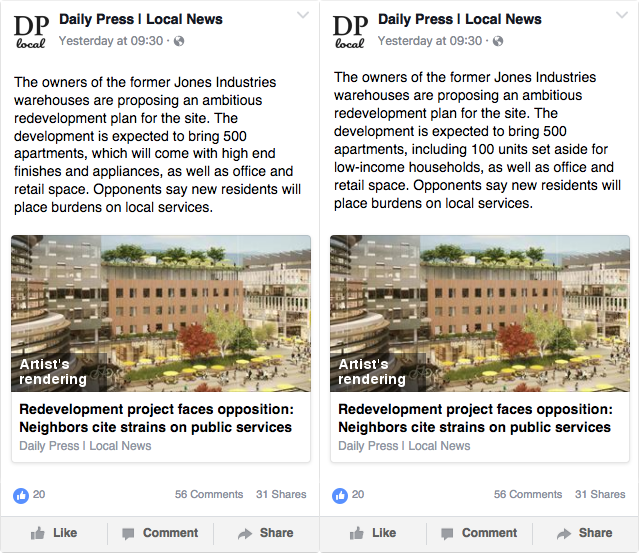
\includegraphics[width=.85\textwidth]{e_treatment}
  }
  \end{measuredfigure}
  \begin{tablenotes}[flushleft]
    \item \hspace{-.2em}\emph{Notes:} Respondents are shown a graphic for either the ``high-end'' project (left) or the mixed-income project (right). The graphic presents information about the project, as well as an artist's rendering of the proposed development.
  \end{tablenotes}
\end{figure}

\noindent Stipulating that the project is a 5-minute drive away (about 2 miles) conveys the idea that the project is near enough to be in the same city as the respondent, but distant enough to be in a different neighborhood. Information about the project is presented as a Facebook post by a local news outlet.  This format allows for a short vignette to be presented together with a rendering of the proposed development in a realistic way; see Figure~\ref{fig:hg_e_treatment}.\footnote{The artist's rendering is taken from documents filed by the developers of the pen factory project, described in Section~\ref{sec:hg_introduction}.}  The text of the vignette reads:

  \begin{quote}
  \begin{SingleSpace}
  The owners of the former Jones Industries warehouses are proposing an ambitious redevelopment plan for the site. The development is expected to bring 500 apartments, [which will come with high end finishes and appliances / including 100 units set aside for low-income households], as well as office and retail space. Opponents say new residents will place burdens on local services.\end{SingleSpace}
  \end{quote}

The graphic primes respondents to consider the potential costs of the project by highlighting in the main text and in the rendering's caption that the new development may strain local public services. The vignette is identical for respondents in both treatment groups, except for the section enclosed within brackets.  Finally, respondents are reminded that
  \begin{itemize}
  \begin{SingleSpace}
    \item A Yes vote will allow developers to build 500 [luxury / mixed-income] apartments, as well as offices and shops.
    \item A No vote will allow developers to build office space and shops, but no new apartments.\end{SingleSpace}
  \end{itemize}

\noindent The reminder emphasizes that the vote is not about whether there will be development -- in both cases, commercial development will proceed -- but whether the project will include residential uses.  Respondents are then asked to state if they will vote yes or no on the project on a four-point Likert scale, with a fifth ``Unsure'' option.  On the same page of the survey, they are asked to justify their decision ``in a few words.'' Although respondents are free to write as few or as many words as they like, the request for a justification encourages respondents to take an additional moment to consider their decision.\footnote{The median length of the open-ended response is 17 words.}

\subsubsection{Summary Statistics}

It is well known that the MTurk population differs from the general population on a number of dimensions \citep[see e.g.][]{huff_who_2015}.  Table~\ref{tab:hg_e_summary_stats} reports demographic characteristics of the sample who completed the survey, and compares these summary statistics to the demographics of several major U.S. cities based on the 2012-2016 American Community Survey 5-year estimates.  The MTurk sample has more females and is younger than the populations of the selected cities, but is similar in some other respects. For example, 40 percent of respondents in the MTurk sample are homeowners, a number comparable to Los Angeles and San Francisco (37 percent of households), as well as Chicago (44 percent).  In terms of education attainment, 55 percent of the MTurk respondents have at least a 4-year college degree, a number higher than most cities, but comparable to San Francisco (53 percent).  Finally, 82 percent of respondents report household income of less than \$100,000, a figure comparable to Chicago (77 percent), Los Angeles (75 percent), and New York (73 percent). Because population characteristics differ from city to city, I do not weight observations to reflect any particular target population.

\begin{table}
  \begin{threeparttable}
  \caption{Summary Statistics and Comparison to Major Cities}
  \label{tab:hg_e_summary_stats}
  \footnotesize
  \begin{tabularx}{\textwidth}{lXXXXXX}
    \hline
     & MTurk & Boston & Chicago & LA & NYC & SF \\ \hline
  Female & 0.58 & 0.53 & 0.52 & 0.51 & 0.53 & 0.49 \\ 
    Age $<$ 35 & 0.53 & 0.47 & 0.38 & 0.36 & 0.35 & 0.35 \\ 
    Age $>$ 54 & 0.09 & 0.25 & 0.28 & 0.28 & 0.31 & 0.30 \\ 
    Homeowner & 0.40 & 0.35 & 0.44 & 0.37 & 0.32 & 0.37 \\ 
    No college education & 0.08 & 0.34 & 0.40 & 0.43 & 0.43 & 0.25 \\ 
    Some college education & 0.37 & 0.24 & 0.26 & 0.27 & 0.23 & 0.23 \\ 
    Has 4-year college degree & 0.41 & 0.24 & 0.21 & 0.20 & 0.21 & 0.33 \\ 
    Post-graduate degree & 0.14 & 0.17 & 0.13 & 0.10 & 0.13 & 0.20 \\ 
    Income $<$ \$60,000 & 0.55 & 0.51 & 0.57 & 0.56 & 0.53 & 0.37 \\ 
    Income between \$60-99,000 & 0.27 & 0.18 & 0.20 & 0.19 & 0.20 & 0.17 \\ 
    Income between \$100-\$149,000 & 0.11 & 0.15 & 0.12 & 0.12 & 0.13 & 0.17 \\ 
     \hline
  \end{tabularx}
  \begin{tablenotes}[flushleft]
    \item \hspace{-.2em}\emph{Notes:} Summary statistics for major cities are based on the American Community Survey 2012-2016 5-year estimates.
  \end{tablenotes}
  \end{threeparttable}
\end{table}

\subsection{Results}

\subsubsection{Measuring Liberalism and Localism} 

Responses to the twelve attitudinal statements are used to estimate the structure of political ideology with respect to local public policy.  I convert the responses on the Likert agree-disagree scale to continuous variables ranging from 1 to 4, with ``No opinion'' given a value of 2.5.  Each variable is then scaled to have mean 0 and unit variance.  I  apply principal components analysis (PCA) on responses to the statements. PCA transforms a set of possibly correlated observed variables into a set of orthogonal latent variables, or principal components (PCs).  Each component is a linear combination of responses to the attitudinal statements. To give substantive meaning to the components, or latent variables, I inspect the factor loadings, or weights, for each of the statements.  I pay particular attention to the loadings for two families of statements.  The liberalism family includes the following statements:
  \begin{itemize}\begin{SingleSpace}
    \item The distribution of money and wealth in this country today is fair.
    \item The government should not concern itself with reducing the income difference between the rich and the poor.
    \item Our government should redistribute wealth through higher taxes on the rich.
    \item Everyone born in this country has an equal chance to succeed in life, whether their family is rich or poor.
  \end{SingleSpace}\end{itemize}

\vspace{1em}The localism family includes the following statements:
  \begin{itemize}
    \begin{SingleSpace}
    \item Local government should focus on helping local businesses do well, rather than attracting new firms to the area.
    \item Every resident of a town or city should have an equal say on local issues, whether they just arrived or are long-time residents.\end{SingleSpace}
  \end{itemize}

% Principal components
\begin{figure}[p]\centering
  \caption{Distribution of Attitudes across Liberalism and Localism Categories}
  \label{fig:hg_e_pc}
  \begin{measuredfigure}
  \makebox[\linewidth]{%
  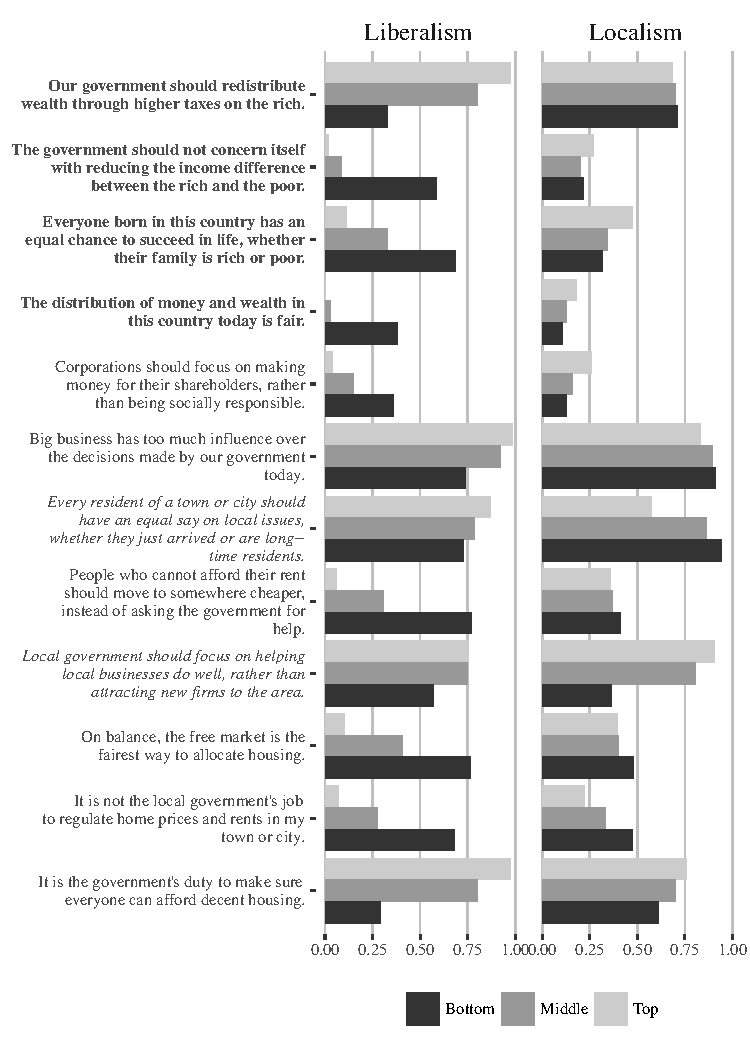
\includegraphics[width=.85\textwidth]{e_pc}
  }
  \end{measuredfigure}
  \begin{tablenotes}[flushleft]
    \item \hspace{-.2em}\emph{Notes:} The figure shows the proportion of respondents who agree with each statement, conditional on liberalism and localism score terciles.  Error bars indicate 95\% confidence intervals. Respondents at different ends of the liberalism scale are differentiated by responses to statements about economic equality and redistribution (in bold). Respondents at different ends of the localism scale are differentiated by responses to statements about local community (in italics). 
  \end{tablenotes}
\end{figure}

\vspace{1em}Liberalism and localism scores are the principal components that most heavily weigh responses in the respective families.  To understand what these scores mean substantively, I show how the scores correspond to raw responses to each attitudinal statement. For each attribute, liberalism and localism, I categorize respondents into terciles based on their scores, and report the proportion of respondents in each tercile who agree or disagree with each statement.  The left column of Figure~\ref{fig:hg_e_pc} reports proportions agreeing, conditional on liberalism scores.  Consider, for example, responses to the first statement, ``Our government should redistribute wealth through higher taxes on the rich.''  97 percent of respondents in the top liberalism tercile (those with the highest scores) agree with this statement, compared to 33 percent of respondents in the bottom tercile.  In contrast, 58 percent of respondents in the bottom liberalism tercile agree with the statement that ``The government should \emph{not} concern itself with reducing the income difference between the rich and the poor,'' compared to 1 percent of those in the top tercile. The conditional distributions of the responses demonstrate that liberalism scores differentiate respondents in favor of economic equity and redistributive social policies from those opposed to such policies.

The right column of Figure~\ref{fig:hg_e_pc} likewise reports the proportions of respondents agreeing to each statement conditional on the localism scores.  Respondents in the highest and lowest terciles for localism differ most significantly in their responses to statements in the localism family. For example, only 58 percent of respondents in the top tercile (highest localism score) agree that ``Every resident of a town or city should have an equal say on local issues, whether they just arrived or are long-time residents,'' compared to 94 percent of those in the lowest tercile.  Similarly, 91 percent of respondents in the top tercile agree that ``Local government should focus on helping local businesses do well, rather than attracting new firms to the area,'' compared to only 36 percent of those in the bottom tercile.  The differences in the responses to statements in the liberalism family, on the other hand, are relatively small.  69 percent of those in the top localism tercile agree that ``Our government should redistribute wealth through higher taxes on the rich,'' a proportion similar to the 71 percent of those in the bottom tercile who agree. 

Note that the type of localism described by this principal component does not necessarily incorporate a heightened concern for displacement.  36 percent of respondents in the top localism tercile agree that ``People who cannot afford their rent should move to somewhere cheaper, instead of asking the government for help,'' only marginally lower than the 41 percent in the bottom tercile who agree. Concern for displacement -- more precisely, support for social policies to mitigate displacement risk -- is instead incorporated into the liberalism component. Put another way, cosmopolitans and localists alike may support (or oppose) anti-displacement legislation. Rather, what divides cosmopolitans and localists is the belief that locals -- long-time residents and (to a lesser extent) legacy businesses -- should be given priority over newcomers and outsiders, whether in terms of political voice or economic development initiatives.  

Table~\ref{tab:hg_e_lib_loc_regression} presents estimates for linear regressions of liberalism and localism on gender, race, age, education, income, and housing status. Socioeconomic variables are associated with liberalism with the expected signs; for instance, liberalism decreases with income and is lower among homeowners compared to renters. However, income and homeownership are not statistically significant predictors of localism. Instead, education turns out to be significantly predictive of localism. All else equal, respondents who do not have a college degree have higher localism scores on average than those with college degrees.  On its face, this finding could be explained by geographic mobility.  That is, respondents with higher education attainment may be less likely to express localist attitudes because they are more geographically mobile and hence more likely to be newcomers now or in the future.  However, other indicators of geographic mobility, such as income, homeownership, or whether the respondent is a long-time resident in her current town or city, are not associated with localism. Alternatively, education may be associated with localism because the college experience fosters interaction within more diverse and cosmopolitan social networks \citep{case_social_1989,chandler_social_2001-1}. These results therefore suggest that localism may be driven by cultural or ideational mechanisms rather than economic self-interest.

% in a manner analogous to the formation of attitudes toward immigration or cross-national cooperation (see e.g. the discussion in \citealt{hainmueller_public_2014} and \citealt{bechtel_preferences_2014}). To be clear, I do not claim that localism is like holding anti-immigration or isolationist attitudes. Rather, my claim is that localism is a type of ideational or cultural belief, rather an expression of economic self-interest.

% Duration of residence is not a key predictor, see Fischel p. 12.

% Predictors

\begin{table}
  \caption{Predictors of Liberalism and Localism}
  \label{tab:hg_e_lib_loc_regression}
  \begin{threeparttable}
  \footnotesize
  \begin{tabularx}{\linewidth}{X}
  \centering

\begin{tabular}{@{\extracolsep{5pt}}lcc} 
\\[-1.8ex]\hline 
\hline \\[-1.8ex] 
 & \multicolumn{2}{c}{\textit{Dependent variable:}} \\ 
\cline{2-3} 
\\[-1.8ex] & Liberalism & Localism\\
\\[-1.8ex] & (1) & (2)\\ 
\hline \\[-1.8ex] 
 Female & 0.454$^{}$ & 0.088$^{}$ \\ 
  & (0.095) & (0.044) \\ 
  & & \\ 
 Non-white & 0.186$^{}$ & 0.300$^{}$ \\ 
  & (0.111) & (0.052) \\ 
  & & \\ 
 Age < 35 & 0.197$^{}$ & 0.242$^{}$ \\ 
  & (0.101) & (0.047) \\ 
  & & \\ 
 No 4-year college degree & $-$0.266$^{}$ & 0.173$^{}$ \\ 
  & (0.103) & (0.048) \\ 
  & & \\ 
 Post-graduate degree & 0.053 & $-$0.089 \\ 
  & (0.146) & (0.068) \\ 
  & & \\ 
 Income < \$60,000 & 0.306$^{}$ & 0.077 \\ 
  & (0.115) & (0.053) \\ 
  & & \\ 
 Income \$100-150,000 & $-$0.280$^{}$ & $-$0.025 \\ 
  & (0.163) & (0.076) \\ 
  & & \\ 
 Income > \$150,000 & $-$0.434$^{}$ & $-$0.167 \\ 
  & (0.251) & (0.117) \\ 
  & & \\ 
 Homeowner & $-$0.616$^{}$ & $-$0.074 \\ 
  & (0.107) & (0.050) \\ 
  & & \\ 
 Resident > 4 years & 0.165 & 0.062 \\ 
  & (0.103) & (0.048) \\ 
  & & \\ 
 5-year HPA > median & 0.163$^{}$ & 0.021 \\ 
  & (0.096) & (0.045) \\ 
  & & \\ 
 Constant & $-$0.338$^{}$ & $-$0.370$^{}$ \\ 
  & (0.172) & (0.080) \\ 
  & & \\ 
\hline \\[-1.8ex] 
Observations & 1,941 & 1,941 \\ 
R$^{2}$ & 0.062 & 0.064 \\ 
Adjusted R$^{2}$ & 0.056 & 0.059 \\ 
\hline 
\hline \\[-1.8ex] 
\end{tabular} 

  \end{tabularx}
  \begin{tablenotes}[flushleft]
    \item \hspace{-.2em}\emph{Notes:} OLS estimates of linear models for liberalism and localism. Numbers in parentheses report standard errors. Base category for education is 4-year college degree; base category for income is \$60-100,000; median 5-year home price appreciation (HPA) is based on Zillow data, median of 100 largest cities. ``Resident > 4 years'' means respondent has lived in the current town or city for 5 or more years.
  \end{tablenotes}
  \end{threeparttable}
\end{table}

\subsubsection{Support for Redevelopment Projects}

Before turning to the relationship between political beliefs and support for redevelopment projects, I discuss a simple model of support in which voters prefer the type of project (high-end or mixed-income apartments) that maximizes narrow economic benefits for themselves.  In this model, renters at each income level prefer the project type that produces more housing units at their income level.  The reason is that an increase in the supply of housing units in a given market segment decreases rents for that type of housing.  This model hence predicts that lower-income renters prefer the mixed-income project over the high-end apartments, whereas high-income renters would prefer the converse.  Homeowners prefer the project type that leads to a greater increase (or smaller decline) in home prices.  All else equal, homeowners across income groups should not differentially prefer one project type over another.  Suppose, however, that lower-income homeowners live in neighborhoods with lower home prices, compared to the neighborhoods in which high-income homeowners live. Then, lower-income homeowners should prefer the high-end project over the mixed-income project, to the extent that the mixed-income project would introduce new lower- and middle-income housing units into the housing stock and depress home prices in the lower-income market segment.

% Figure: Income and tenure. Inconsistent with narrow self-interest.
\begin{figure}[tb]\centering
  \caption{Support for Project by Household Income and Tenure}
  \label{fig:hg_e_income_tenure}
  \begin{measuredfigure}
  \makebox[\linewidth]{%
  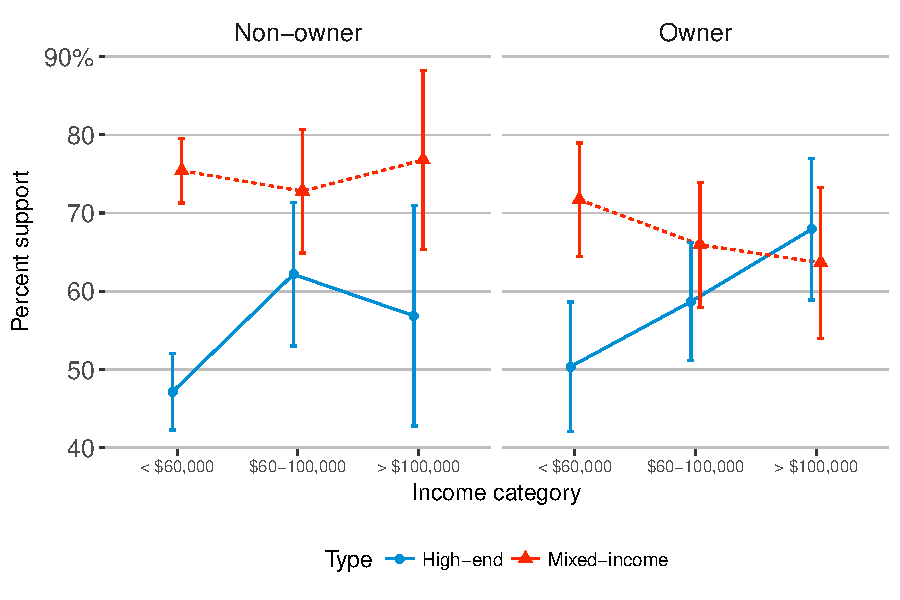
\includegraphics[width=.85\textwidth]{e_income_tenure}
  }
  \end{measuredfigure}
  \begin{tablenotes}[flushleft]
    \item \hspace{-.2em}\emph{Notes:} The figure shows the proportion of respondents that support each project type, for each income category within each housing tenure type (non-owners and homeowners). Error bars indicate 95\% confidence intervals.
  \end{tablenotes}
\end{figure}

Figure~\ref{fig:hg_e_income_tenure} reports support for each project type among non-owners (renters) and owners across three income groups.  Support is defined as choosing ``Definitely yes'' or ``Probably yes'' for the vote choice question.  High-income renters are more likely to support the high-end project, compared to lower-income renters.  However, contrary to the predictions of the model sketched out above, renters at every income level prefer the mixed-income project to the high-end project.  Lower-income homeowners are also more likely to support the mixed-income project compared to the high-end project. Furthermore, homeowners' support for the high-end project is positively associated with their income, a pattern that is not well-explained by narrow, short-run economic self-interest.

% Figure: Bivariate LOESS, liberalism and localism (hetero. treatment efx for lib, decr. support for loc.)
\begin{figure}[tb]\centering
  \caption{Support for Project by Liberalism and Localism Scores}
  \label{fig:hg_e_lib_loc}
  \begin{measuredfigure}
  \makebox[\linewidth]{%
  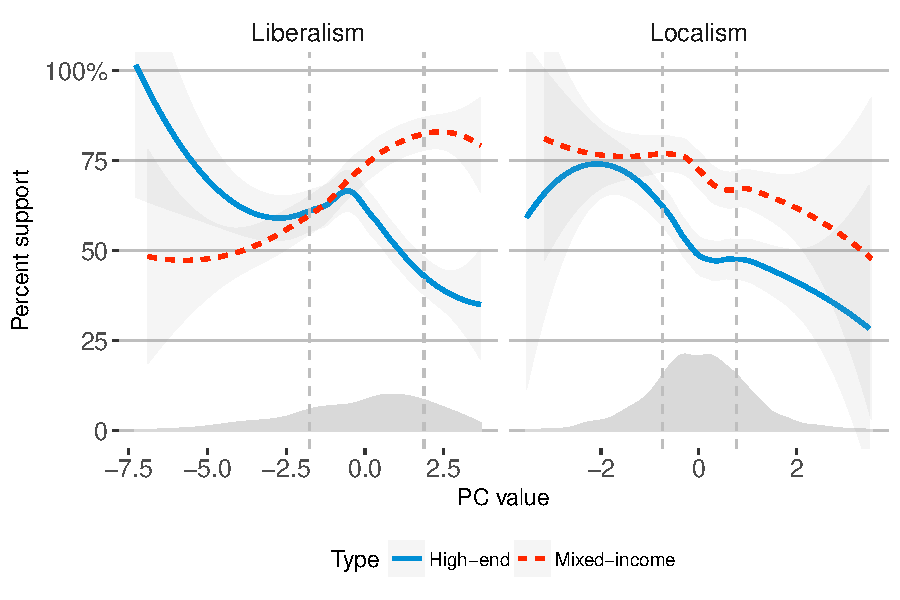
\includegraphics[width=.85\textwidth]{e_lib_loc}
  }  
  \end{measuredfigure}
  \begin{tablenotes}[flushleft]
    \item \hspace{-.2em}\emph{Notes:} The figure shows the bivariate relationship between respondents' support for each project type, and liberalism and localism scores. Lines are LOESS curves.  Density curves at the bottom of the plots show the distribution of the scores; note that the probability densities are scaled for aesthetic reasons and do not correspond to the tick marks on the y-axis. Shaded areas indicate 95\% confidence intervals. The vertical dashed lines represent the 20th and 80th percentiles for the respective scores.
  \end{tablenotes}
\end{figure}

Data from the survey experiment exhibit patterns consistent with the ideology-based theory discussed in Section~\ref{sec:hg_theory}.  As Figure~\ref{fig:hg_e_lib_loc} shows, support for the mixed-income project increases with liberalism (left panel). The predicted probability of supporting the mixed-income project increases from 60 percent for a voter with a liberalism score at the 20th percentile, to 82 percent for a voter with a liberalism score at the 80th percentile, an increase of 22 percentage points.\footnote{Predicted probabilities are computed based on a LOESS fit.}  The positive association between liberalism and support for the  project is reversed when the apartments are all high-end.  As a result, the treatment effect (i.e. the relative preference for the mixed-income over the high-end project) increases from -1 percentage point (statistically insignificant) to 39 percentage points over the same range of liberalism (from the lowest to the highest quintile). Among liberal voters, setting aside units for lower-income households has a substantively and statistically significant effect on support for the mixed-use project. Whereas only a minority of liberal voters support the mixed-use over the commercial-only project when all apartments are marketed as high-end, an overwhelming majority of such voters support the mixed-income project.\footnote{The relationship between liberalism and support for each type of project may be amplified due to question ordering effects. Because respondents were asked about their political attitudes immediately prior to the treatment module, they may be primed to express support for the projects in line with their previously stated beliefs. To the extent that political campaigns also work to activate liberal or localist attitudes prior to an election, this critique is not a concern for external validity.}

In contrast to liberalism, localism is negatively associated with support for both mixed-income and high-end projects.  The predicted probability of supporting the mixed-income project decreases from 77 percent for a voter with a localism score at the 20th percentile, to 67 percent for a voter with a score at the 80th percentile, a decline of 10 percentage points.   Likewise, the probability of supporting the high-end project decreases from 62 percent to 48 percent over the same range, or a decline of 14 percentage points.  While it is not a prediction made by the model, it is intriguing that strong cosmopolitans -- respondents at the extreme low end of the localism scale -- do not appear to discriminate between the types of project.  For example, at the 1st percentile of localism, the predicted probability of supporting the mixed-income project is 77 percent, compared to 74 percent for the high-end project, a difference of 3 percentage points (not statistically distinguishable from zero at the 95\% confidence level; see Figure~\ref{fig:hg_e_ate}).  Cosmopolitans -- respondents who tend to be open to both newcomers and new businesses -- are equally happy to support both high-end and mixed-income developments. The finding is consistent with the expansive view of ``community'' espoused by proponents of residential development at all income levels.

% Liberalism and localism indexes

The estimated relationships between support for the projects and liberalism and localism may be confounded by unobserved variables. For example, given that lower-income individuals tend to be more liberal, the positive association between support for a mixed-income project and liberalism may simply reflect the effect of income.  I estimate linear models of support for each type of project, controlling for gender, race, age, education, income, housing tenure, and local home price appreciation.  Figure~\ref{fig:hg_e_lib_loc} suggests that the relationships between support and the two ideological dimensions can be approximated with a quadratic function, so I include squared terms for liberalism and localism in the models.  Table~\ref{tab:hg_e_support_regression} shows that the associations between political beliefs and support for each project type are robust to the inclusion of covariates.

% Figure: Contour, H and M

\begin{figure}[t]
  \caption{Contour Plots of Support for Project by Project Type}
  \label{fig:hg_e_contour}
  \begin{measuredfigure}
  \makebox[\linewidth]{%
  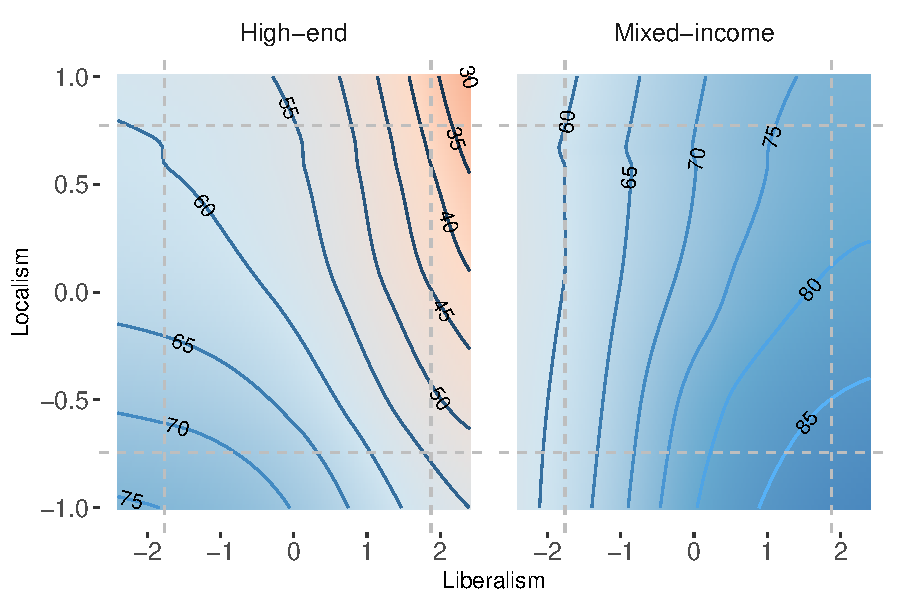
\includegraphics[width=.85\textwidth]{e_contour}
  } 
  \end{measuredfigure}
  \begin{tablenotes}[flushleft]
    \item \hspace{-.2em}\emph{Notes:} The figure shows predicted support for each type of project (high-end or mixed-income housing) as a function of a respondent's liberalism and localism scores, based on LOESS fits with the two predictors.  The vertical and horizontal dashed lines represent the 20th and 80th percentiles for liberalism and localism scores, respectively.
  \end{tablenotes}
\end{figure}

Figure~\ref{fig:hg_e_contour} reports the combined effect of liberalism and localism on support for each type of project.  Like Figure~\ref{fig:hg_e_lib_loc}, the plots report the predicted probabilities of support for a project based on LOESS fits; the difference is that in these plots, support is modelled as a function of both liberalism and localism.  The figure shows that liberal localists are least supportive of the high-end project (top right corner of the left panel), whereas liberal cosmopolitans are most supportive of the mixed-income project (bottom right corner of the right panel). 

% More interestingly, the plots show how localism is differentially associated with support for the projects conditional on liberalism. Consider the predicted probabilities of support for the high-end project.  Among respondents at the 20th percentile of liberalism (left vertical line), moving from the 20th to 80th percentile of localism (from the bottom to the top horizontal line) decreases support for the project from 72 to 60 percent, a decline of 12 percentage points. Among respondents at the 80th percentile of liberalism (right vertical line), support decreases from 54 to 38 percent, a decline of 16 percentage points. The localism gradient of support for the high-end project is steeper among liberals than conservatives (the same is true for the mixed-income project).  Localism is an especially potent force in shaping attitudes toward development in liberal cities, because high land and construction costs orient private development toward high-end (or market-rate) development, and localism can tip the scale away from support for development. I discuss implications for practice in the conclusion.

In this section, I document how housing growth preferences are shaped by individuals' political beliefs.  I focus on two dimensions of political ideology specific to local public policy that I call liberalism and localism.  The sign of the association between liberalism and support for housing growth is conditional on the type of housing growth being proposed, whereas localism is negatively associated with support regardless of type. The treatment effect of a mixed-income project -- that is, the preference gap for a mixed-income project over a high-end project -- is positive and substantively large among liberals, but small and statistically insignificant among conservatives (and negative among very conservative individuals).  The preference gap for the mixed-income project is positive across most values of localism, but strong cosmopolitans tend to be equally supportive of both projects.

\section{San Francisco's Land Use Ballot Measures, 2007-2016}\label{sec:hg_sf}

One concern about the survey experiment is that it does not use actual behavior as its outcome variable.  Survey respondents may support or oppose a project simply as a way to express underlying attitudes, given that there are no real-life costs or benefits at stake.  This section bridges the gap between reported preferences and observed political behavior by studying voting outcomes in a city where liberalism and localism shape responses to a housing affordability crisis.

In this section I exploit rich elections data on housing and land use ballot measures in California.  A report published by California's Legislative Analyst's Office in 2015 enumerated the causes of housing supply shortfalls in the state's coastal areas, beginning with ``Community Resistance to New Housing'' \citep{alamo_californias_2015}.  The report highlighted the effect of local ballot measures on limiting development, noting that ``California's high degree of voter involvement in land use decisions appears to be unique'' (p. 17).  I focus on one city, San Francisco, where voters have repeatedly gone to the polls to make decisions on land use.  The goals of this study are to discover the latent structure of political preferences that undergirds observed vote outcomes, ascertain if any dimensions of this structure can be plausibly described as liberalism and localism, and finally estimate the association between these latent factors and support for redevelopment projects.

San Francisco provides a useful empirical setting for two reasons. First, San Francisco is an exemplar of a set of high-wage, high-growth cities in which land use and housing are highly regulated. These cities include large urban cores like New York and Los Angeles, as well as smaller cities like Seattle, Portland, Boulder, and Austin. Similarities in the liberal leanings of these cities and the political institutions governing land use suggest the generalizability of findings from San Francisco to these other settings (as \citealt{hankinson_when_2018} also notes). Second, San Francisco's tradition of direct democracy, especially in the domains of land use and housing, generates a rich set of fine-grained behavioral measures that can be used to recover latent ideological dimensions, much like roll-call votes.  Ballot initiatives and referenda, also called propositions or measures, are the main instruments of direct democracy.  The next section provides additional background on ballot measures.

\subsection{Setting}

\subsubsection{Land Use and Housing Ballot Measures}

California's state constitution empowers its cities to pass ordinances on traditional municipal matters without prior authorization from the state legislature, to the extent that such ordinances do not conflict with a general state law (Article XI, section 7).  The empowerment of localities by the state to pass laws and ordinances without a prior delegation of authority from the state is known as home rule, and the basis for such laws and ordinances is founded in local police power, which gives local governments the right to act in a way that promotes the health, safety, and general welfare of the community.\footnote{See for example the discussions in \citet[pp.19ff]{fischel_homevoter_2001} and \citet[pp.70ff]{berman_local_2015}.}  Land use regulation, in particular, has its basis in police power.  

Citizens can influence local public policies in several ways.  They can elect or lobby public officials.  In some states, including California, they can also petition to place legislation on the ballot to be voted on directly by the electorate.  The same process also allows citizens to repeal legislation passed by elected officials.  In California, the use of such ballot initiatives and referenda -- also called ballot measures or ballot propositions -- to shape local land use planning began in the 1970s \citep[p. 244]{fulton_guide_2012}.  Initiatives restricting growth first appeared on local ballots in the San Francisco area, but gradually spread to localities in Southern California over the course of the 1970s and 1980s.

The most common type of land use ballot measures restrict (or ease restrictions on) development.  For example, Proposition M in San Francisco's 1986 November elections placed an annual cap on the square footage of office space in high-rise buildings; subsequent measures have sought to amend or circumvent this cap.  Measures could also seek to impose development moratoria in certain neighborhoods.  Other measures have more subtle effects on growth. For example, parking requirements stipulate the minimum number of parking spaces developers would need to include in new projects. Reduced minimum parking requirements, especially in neighborhoods well served by public transit, can reduce per-unit costs for developers and increase housing density. Measures that seek to amend parking requirements thus have a subtle but direct effect on housing growth.

A second type of measures introduces or amends procedural barriers to development. Such measures might mandate voter approval for zoning changes or increases to height limits.  Conversely, a measure might require the city to let a project proceed so long as it meets certain criteria, allowing the project to circumvent hearings, appeals, and petitions.  Another example would be a measure that requires publicly-funded projects, such as affordable housing developments, to receive a minimum number of bids or proposals. To the extent that such projects are complex and require specialized expertise, such a mandate may limit the number of types of projects that can be built.

A third type of ballot propositions is fiscal measures. Such measures could require that a proportion of tax revenues be set aside for specific uses, such as acquiring or preserving open space, affordable housing, and so on.  These measures do not raise new revenue, but provide dedicated funding sources for certain public projects. Voter approval is also needed for bond issues. Over the last two decades, San Francisco voters have gone to the polls thrice -- in 2002, 2004, and 2015 -- to approve new bond issuance to fund affordable housing programs.

A fourth type of propositions relates to voter approvals for specific projects. These projects are described in more detail in the following section.  The specifics of each project require additional exposition because of our theorizing that citizens' political beliefs are differentially associated with support for redevelopment, depending on the characteristics of each redevelopment project.

\subsubsection{Redevelopment Projects}\label{sec:hg_g_redev}

Since 2008, San Francisco's voters have voted on six measures related to approvals for four redevelopment projects. Figure~\ref{fig:hg_g_devs} indicates the locations of these projects. The projects were the subjects of ballot measures either because existing local legislation requires voters to approve zoning or height limit changes in specific situations (as with the Hunters Point Shipyard, Pier 70, and Mission Rock), or because proponents or opponents -- or both -- collected sufficient signatures for a petition to put a measure on the ballot (as with the 8 Washington project).  I describe the projects in more detail below, noting in particular whether each project was perceived as being sufficiently attentive to housing affordability or not.

\begin{figure}[tb]\centering
  \caption{Project-specific Ballot Measures}
  \label{fig:hg_g_devs}
  \begin{measuredfigure}
  \makebox[\linewidth]{%
  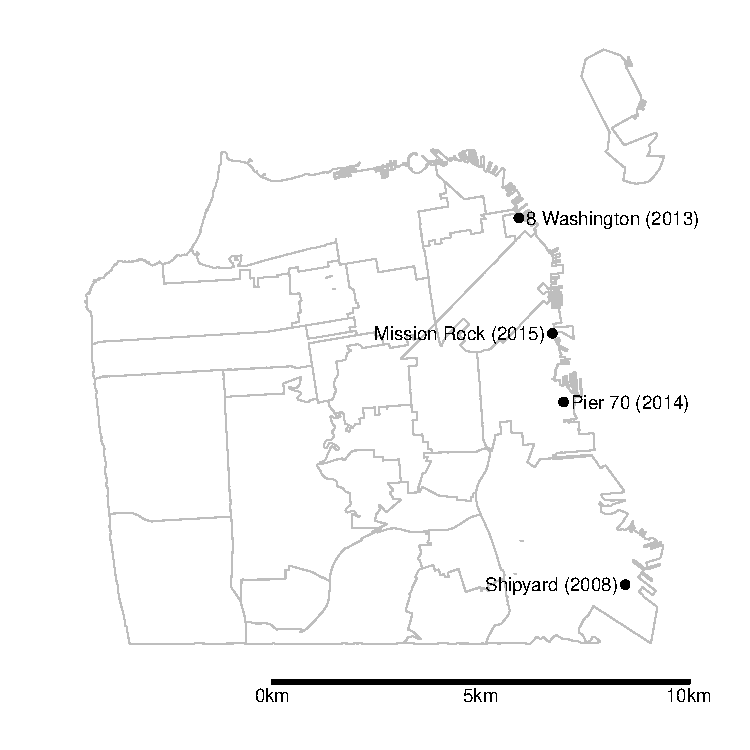
\includegraphics[width=.7\textwidth]{g_devs}
  }
  \end{measuredfigure}
  \begin{tablenotes}[flushleft]
    \item \hspace{-.2em}\emph{Notes:} The figure shows the locations of four projects that sought voter approval between 2008 and 2015.
  \end{tablenotes}
\end{figure}

\paragraph{Hunters Point Shipyard} In June 2008, San Francisco voters voted on a proposed framework for the redevelopment of the Hunters Point Naval Shipyard and Candlestick Point (Measure G). The proposition was placed on the ballot because the site included an existing stadium, which together with its surrounding parking lots were classified as open space. Since city laws already required voter approval to change the zoning of open space for other uses, the mayor took the opportunity to seek a broad mandate for the redevelopment of the site. The proposal envisioned the production of 8,500 to 10,000 new housing units. The proposition text did not, however, specify the affordability levels of these units.\footnote{A Community Benefits Agreement signed by the developer and community organizations in May 2008 committed the developer to pricing at least 32 percent of units at affordable levels. See \url{https://d10benefits.org/wp-content/uploads/2013/01/lennar_ad10_ccba_executed-1.pdf}.} The language of Measure G was perceived by some as being relatively favorable to developers.\footnote{San Francisco distributes voter pamphlets to voters that contain arguments and endorsements contributed by each proposition's proponents and opponents. In their official argument against Measure G, opponents begin with the claim that ``Proposition G makes big promises but doesn't guarantee affordable housing, jobs for local residents, or any more parkland than already exists. Proposition G is a sweetheart deal for Lennar, an out-of-state developer that has already spent over \$1,000,000.00 on its political campaign. \ldots{}. Transit `improvements' promised by Lennar will primarily benefit new luxury condo owners, not the rest of Bayview.''}  Partly in response to perceived slipperiness in Measure G as regards the project's commitment to housing affordability, opponents to the project gathered sufficient signatures to place a competing measure on the ballot (Measure F). The competing measure required the project to set aside at least 50 percent of new housing units as affordable housing, with varying levels of affordability benchmarked to median household income in the city. Measure G passed with 63 percent of the vote; Measure F failed with 37 percent. About 160,000 votes were cast.

\paragraph{8 Washington} In 2012, the San Francisco Board of Supervisors passed an ordinance that increased height limits for a site on the city's eastern waterfront, as part of the approvals for a recreational, retail, and residential development known as 8 Washington Street. Local law allows citizens to reaffirm or overturn the Board's decision in a referendum, and opponents of the height limit increase gathered sufficient signatures to put the question to voters in the November 2013 local elections (Measure C). Although Measure C was narrowly focused on the question of height limits, overturning the height limit increases would effectively prevent the project from proceeding. In response, proponents of the project put a competing measure on the ballot (Measure B) for voters to approve the project.  The project as proposed would have added 134 market-rate units to the housing stock. In addition, the developer pledged a \$11 million contribution to the city's affordable housing fund. Although opponents' main complaint addressed the height limit increase, they also noted the absence of on-site affordable housing, and claimed that the new ``luxury condos'' would cost \$5 million on average.  About 125,000 votes were cast, and the project was rejected by about 65 percent of voters. The developer abandoned the project in 2016.

\paragraph{Pier 70 and Mission Rock} In June 2014, voters passed a ballot measure (Measure F) mandating voter approval for height limit increases on certain sites along the eastern waterfront. The measure directly affected two developments, Pier 70 and Mission Rock.  Pier 70's developer, which had been engaging interest groups and community members on its plans for the site since 2011, felt sufficiently confident in its level of community support to put the project on the November 2014 ballot \citep{kuwada_shaping_2015}.\footnote{Incidentally, Pier 70's developer is Forest City -- the same firm that developed University Park, described at the beginning of Section~\ref{sec:hg_exp}.} The project would add between 1,000 and 2,000 housing units to the city, with the developer committing to price 30 percent of the units at levels affordable to low- and middle-income households. The proportion of affordable housing units exceeded the 12 percent affordable requirement that was city law at the time. The Mission Rock project, which was on the November 2015 ballot, committed to an even higher proportion of affordable housing. The project envisioned 1,000 to 1,950 new housing units, of which at least 40 percent would be affordable to low- and middle-income households. Endorsements of the two measures published in official voter pamphlets underline the high proportion of affordable housing units proposed for these two projects.  Both measures won at the ballot box with similar margins -- 73 to 74 percent `Yes' votes -- on over 200,000 votes cast.

\subsection{Data and Measurement}

\subsubsection{Dataset}

I construct a novel panel dataset of voting outcomes for about 600 precincts in San Francisco, California, on 19 city-level housing and land use related ballot measures presented to voters between 2007 and 2016. The set of measures used in the analysis was defined by including all measures belonging to the ``land use'' category as coded by researchers at the California Elections Data Archive, a project co-sponsored by the Office of the California Secretary of State.\footnote{The project's website is at \url{http://www.csus.edu/isr/projects/ceda.html}.} The initial list of measures was then supplemented by measures that included the words ``land'' or ``development'' and are clearly related to land use. The latter set of measures mostly relate to affordable housing issues and approvals for specific projects.

The San Francisco Department of Elections publishes vote counts for each ballot proposition at the precinct level. In 2016, about 850 voters were registered in each precinct on average. Because precinct boundaries may change from election to election, I create a panel by matching precincts from a reference election (specifically the 2012 general election) to precincts from other elections based on the proportion of spatial overlap between precincts. In other words, each precinct from the 2012 general elections is matched to a precinct in every other elections to create the panel.

\subsubsection{Measures of Liberalism and Localism}

Similar to the study in Section~\ref{sec:hg_exp}, I apply principal components analysis to observed precinct-level vote outcomes to generate uncorrelated latent dimensions. I then inspect the loadings for each principal component to determine if any of the components can be plausibly interpreted as measuring liberalism or localism.  The interpretation of the components is complicated by the fact that unlike attitudinal survey questions, which researchers can design to tap specific political attitudes, ballot measures often do not map clearly onto an ideological space. For example, a ballot measure that updates the city charter to include lower-income constituencies in the policymaking process may be viewed as raising procedural barriers to development, or an effort to ensure economically equitable development outcomes, or both. Voters' interpretations of the ballot measures may also be guided by how the measures are framed by elites, such as politicians, community leaders, local think-tanks, or neighborhood groups.  The challenge for the researcher is to identify political beliefs that best describe the variation in voting patterns along latent ideological dimensions.

Consistent with prior research in American political behavior, the first component has a clear interpretation as a measure of economic liberalism \citep[e.g.][]{ansolabehere_candidate_2001,treier_nature_2009,tausanovitch_measuring_2013}.  To illustrate the substantive interpretation of this latent dimension, I categorize precincts into terciles according to their PC scores, and report the average vote share by terciles for a selected set of ballot measures (Figure~\ref{fig:hg_e_pc}). Precincts that score highly on the first component are more supportive of ballot measures that have redistributive objectives or have the ostensible intention of protecting economically vulnerable groups (left column of Figure~\ref{fig:hg_e_pc}).  Consider the Affordable Housing Bond measure of 2015, in which voters approved \$310 million of municipal borrowing for housing affordability programs, to be paid down using property tax revenues. Among precincts in the top tercile of PC1 scores, average vote share in support of the measure was 84 percent, compared to 75 percent and 64 percent among precincts in the middle and bottom tercile respectively. The same pattern is observed for the Affordable Housing measure of 2014, which is a non-binding policy declaration stating the city's goal of building or rehabilitating 30,000 homes by 2020, together with affordability targets for these homes. Average vote share in favor of this measure was 76 percent among precincts in the top PC1 tercile, compared to 67 percent and 55 percent in the middle and bottom tercile respectively.\footnote{For both the abovementioned measures, differences between terciles are statistically significant at the $p < 0.01$ level, using robust standard errors clustered at the neighborhood level.}

\begin{figure}[p]\centering
  \caption{Support for Ballot Propositions across Liberalism and Localism Categories}
  \label{fig:hg_g_pc}
  \begin{measuredfigure}
  \makebox[\linewidth]{%
  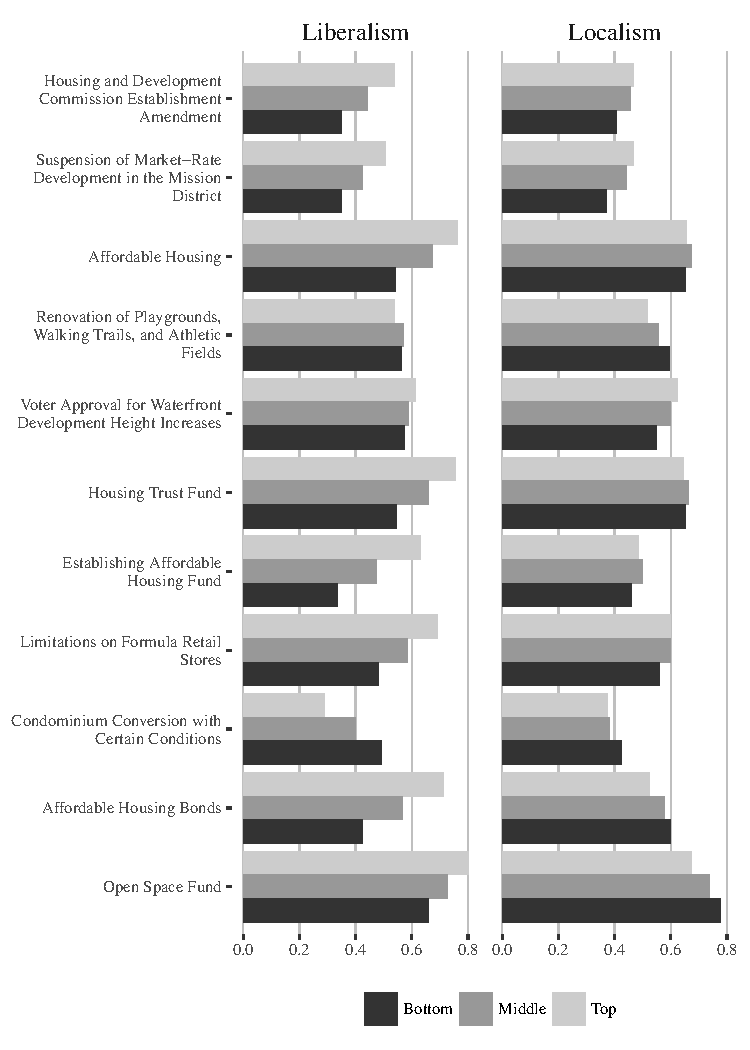
\includegraphics[width=.85\textwidth]{g_pc}
  }
  \end{measuredfigure}
  \begin{tablenotes}[flushleft]
    \item \hspace{-.2em}\emph{Notes:} The figure shows the mean precinct-level vote in favor of each ballot proposition, conditional on liberalism and localism score terciles. Error bars represent 95 percent confidence intervals.
  \end{tablenotes}
\end{figure}

To identify a latent dimension associated with localism, I inspect the loadings to find a component that differentiates precincts on ballot measures that limit or enhance voter control over development.  These measures include November 2014 Measure I, which limits local residents' ability to block improvements to recreational facilities that would at least double the usage of a facility, as well as the aforementioned June 2014 Measure F, which mandates voter approval for height limit increases on certain sites along the eastern waterfront.  Based on this criterion, I select the third component as a measure of localism (right column of Figure~\ref{fig:hg_e_pc}).\footnote{The second component differentiates precincts on measures finely tailored to the San Francisco context -- e.g. allowing billboards in a specific section of the business district -- and does not have obvious generalizable implications.} Although this component explains significantly less variance in the observed vote outcomes compared to the liberalism dimension, it can still be differentiated from subsequent components in terms of the proportion of variance explained (see Figure~\ref{fig:hg_g_scree}). Consider the 2014 ``Renovation of Playgrounds'' measure, which would limit the ability of local communities to block certain public works improvements, so long as the improvements double the use of the public facility. Among precincts in the top tercile of PC3 scores -- the most localist precincts -- the average vote share in support of this measure was 51 percent, compared to 56 percent and 60 percent in the middle and bottom terciles respectively. PC3 also differentiates precincts on the ``Voter Approval for Waterfront Development Height Increases'' measure, for which mean vote shares were 63, 60, and 55 percent for the top, middle, and bottom localism terciles respectively.\footnote{Differences between terciles are statistically significant at the $p < 0.01$ level, using robust standard errors clustered at the neighborhood level.}

The maps in Figure~\ref{fig:hg_g_pc_map} report the values of the liberalism and localism scores for each precinct in San Francisco. The geographic distribution of liberalism (top panel of figure) is consistent with qualitative descriptions of San Francisco's political geography. Observers of the city's politics refer to a ``Conservative C'' that stretches along the wealthy northern edge of the city, bordering the Presidio, down the middle- and upper-class west-side, and along the southern border.\footnote{See for example \url{http://www.dailykos.com/story/2012/11/19/1160963/-A-crash-course-in-San-Francisco-politics}.} Neighborhoods in the center of the city and toward the southeastern edge -- the ``Progressive Core'' -- are on the other ideological pole. Even in a city known for its liberal politics (where neighborhoods are ``conservative'' only to the extent that they are less liberal than other San Francisco neighborhoods), substantive geographic variation exists with respect to preferences over redistributive public policy.

\begin{figure}\centering
  \caption{Geographical Distribution of Liberalism and Localism}
  \label{fig:hg_g_pc_map}
  \begin{measuredfigure}
  \makebox[\linewidth]{%
  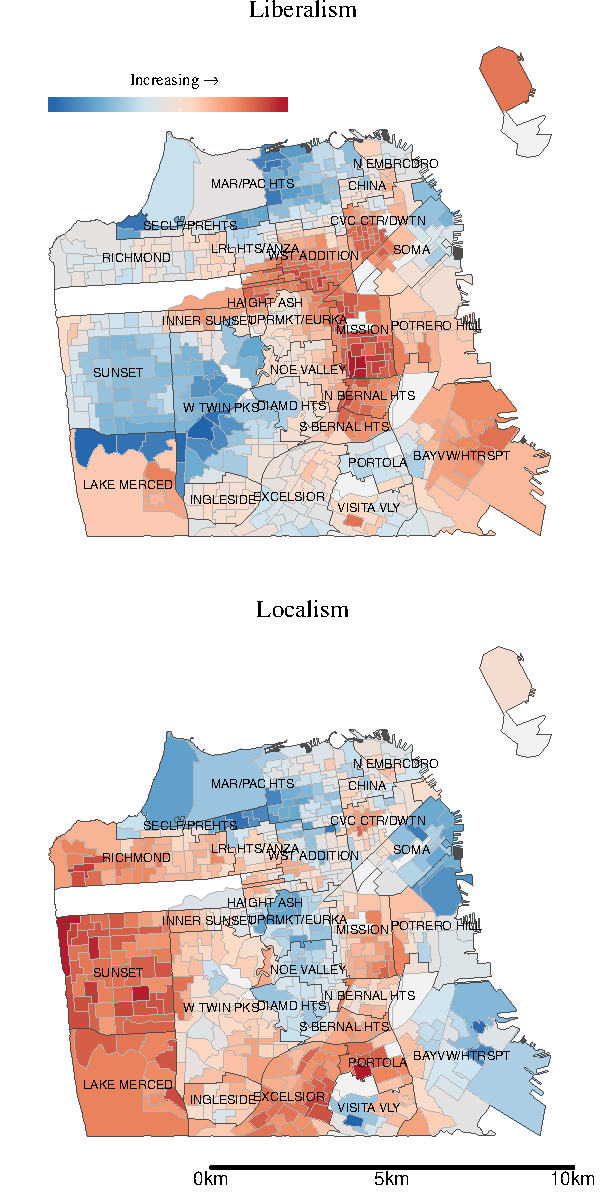
\includegraphics[width=.65\textwidth]{g_pc_map}
  }
  \end{measuredfigure}
  \begin{tablenotes}[flushleft]
    \item \hspace{-.2em}\emph{Notes:} The maps show the liberalism and localism scores for each precinct in San Francisco.
  \end{tablenotes}
\end{figure}

Localism has a different geographic distribution (bottom panel of figure).  Neighborhoods on different ends of the liberalism spectrum can become proximate in terms of localism.  The Mission district, one of the most liberal neighborhoods, looks more similar to the conservative Sunset district on the localism dimension than its liberal neighbors in Noe Valley and the Castro (labelled as \texttt{EURKA} on the map, for Eureka Valley).  On the other hand, the conservative Pacific Heights neighborhood (\texttt{MAR/PAC HTS}) is similar to the Castro in terms of its cosmopolitanism. Figure~\ref{fig:hg_g_libloc_space} visualizes these relationships.

\begin{figure}\centering
  \caption{San Francisco Neighborhoods on a Liberalism-Localism Space}
  \label{fig:hg_g_libloc_space}
  \begin{measuredfigure}
  \makebox[\linewidth]{%
  \includegraphics[width=.65\textwidth]{g_libloc_space}
  }
  \end{measuredfigure}
  \begin{tablenotes}[flushleft]
    \item \hspace{-.2em}\emph{Notes:} The figure locates neighborhoods in San Francisco on a liberalism-localism space, based on median neighborhood scores on each dimension. Neighborhoods that are distant on one dimension may be proximate on another. For example, the Sunset and Mission neighborhoods are on opposite ends of the liberalism dimension, but are nearer to each other in terms of localism.
  \end{tablenotes}
\end{figure}

Categorizing San Francisco's neighborhoods along two dimensions -- liberalism and localism -- allows for a richer understanding of the city's political geography.  Figure~\ref{fig:hg_g_map_types} shows the clustering of neighborhoods based on the interaction of whether they score above or below the median on liberalism (liberal or conservative) and whether they score above or below the median on localism (localist or cosmopolitan).  The theory described in Section~\ref{sec:hg_theory} implies that support for redevelopment projects should vary systematically across the four different categories of neighborhoods.

\subsection{Support for Redevelopment Projects}

\subsubsection{Support By Liberalism-Localism Categories}

In Section~\ref{sec:hg_theory}, I hypothesize that a voter's support for a project should increase with liberalism when new homes are perceived to be equitably distributed, and decrease with liberalism when it is characterized as a high-end project.  Localism, by contrast, should be negatively associated with support for a project regardless of the project type.  In this section, I present results from an analysis of ballot measure outcomes on the four projects described above.

\begin{figure}\centering
  \caption{Support for Project by Liberalism and Localism Categories}
  \label{fig:hg_g_lib_loc}
  \begin{measuredfigure}
  \makebox[\linewidth]{%
  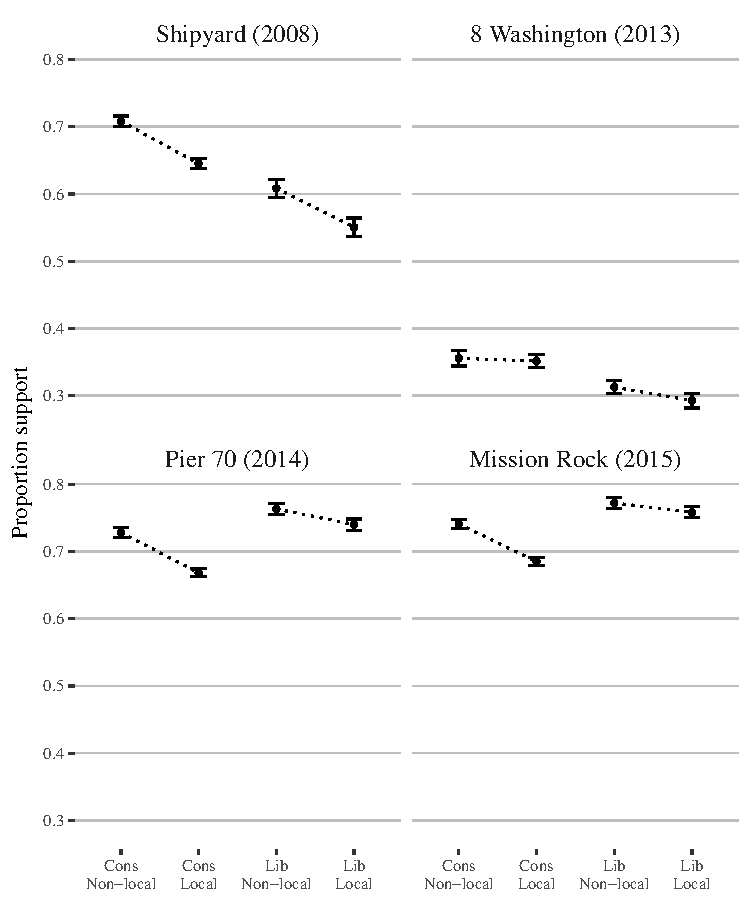
\includegraphics[width=.9\textwidth]{g_lib_loc}
  }
  \end{measuredfigure}
  \begin{tablenotes}[flushleft]
    \item \hspace{-.2em}\emph{Notes:} The figure shows the proportion of respondents that support each project type, for each liberalism-localism category. Error bars indicate 95\% confidence intervals.
  \end{tablenotes}
\end{figure}

I report category mean vote shares for each of the four projects (Figure~\ref{fig:hg_g_lib_loc}). There are four categories of precincts, defined by crossing liberal-conservative types with  localist-cosmopolitan types.  The findings reported in Figure~\ref{fig:hg_g_lib_loc} are consistent with theoretical expectations.  On average, liberal precincts (those with above-median liberalism scores) are less supportive of the Shipyard and 8 Washington projects than conservative precincts.  The pattern is reversed for the Pier 70 and Mission Rock projects, which receive more support from liberal precincts than conservative ones.  As mentioned above, developers for the latter pair of projects committed to setting aside at least 30 percent of newly constructed housing units for low- and middle-income households.  By contrast, opponents to the Shipyard project argued that it ``doesn't guarantee affordable housing,'' and the 8 Washington project included no on-site affordable housing units.  

The dotted lines in the figure connecting each pair of points illustrate how localism is negatively associated with support for projects, regardless of the project type.  When controlling for liberalism, vote shares for cosmopolitan precincts are at least as high as those of localist precincts.  These correlations are robust to the inclusion of controls for homeownership rates and household income (see Table~\ref{tab:hg_g_support_regression}). Finally, Figure~\ref{fig:hg_g_lib_loc} shows that liberalism moderates the relationship between localism and support for new developments, particularly for projects with a more equitable distribution of new homes (bottom pair of panels). Although localist precincts are less supportive of new developments compared to cosmopolitan precincts, the drop-off in support among liberal precincts is smaller compared to that among conservative precincts. These findings suggest that at the margins, affordable housing set-asides can be a means of winning support for new developments from liberal localists.

\subsubsection{Alternative Measures of Liberalism and Localism}

Interpretations of the principal components are subjective. That is, although I show that the first and third components from a principal components analysis of ballot measure outcomes are systematically associated with vote outcomes for redevelopment projects in a manner consistent with expectations from a theory of two-dimensional ideology, interpretations of the components may differ across researchers. To address this concern, I use vote outcomes on individual ballot propositions as measures of liberalism and localism.  I select propositions that express liberalism and localism with the least ambiguity.  To measure liberalism, I use precinct-level vote shares for November 2015 Proposition A. As mentioned above, the proposition sought voter approval to borrow \$310 million for the development and preservation of low- and middle-income housing, as well as financial assistance for middle-income homebuyers. To measure localism, I use vote shares for June 2014 Proposition B, which sought to require voter approval for increasing height limits on waterfront developments.

\begin{figure}[t]
  \caption{Contour Plots of Support for Projects}
  \label{fig:hg_g_contour}
  \begin{measuredfigure}
  \makebox[\linewidth]{%
  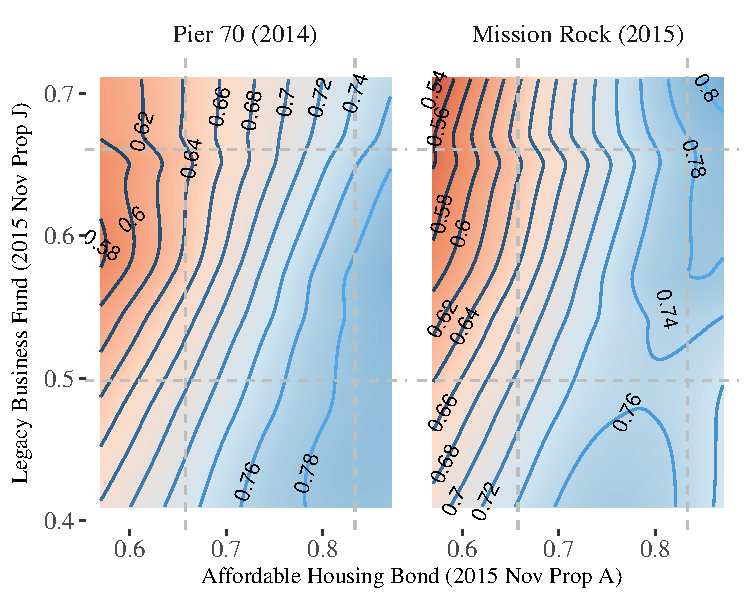
\includegraphics[width=.85\textwidth]{g_contour}
  } 
  \end{measuredfigure}
  \begin{tablenotes}[flushleft]
    \item \hspace{-.2em}\emph{Notes:} The figure reports predicted support for the Shipyard and Mission Rock projects from LOESS estimates.  Levels of predicted support are indicated by colors in the plot as well as labels on the contour lines.  The predictors are the proportion of votes in each precinct supporting November 2015 Prop A (Affordable Housing Bond) and June 2014 Proposition B (Voter Approval for Waterfront Development).  The vertical and horizontal dashed lines represent the 20th and 80th percentiles for the proportion of votes supporting the propositions.
  \end{tablenotes}
\end{figure}


%Proposition J, ``Legacy Business Historic Preservation Fund,'' from the same election.  The fund would provide subsidies to legacy businesses, defined as businesses that have been operating in San Francisco for at least 20 years and ``have significantly contributed to history or identity of a neighborhood.''  The proposition does not raise new taxes or identify funding sources, but clearly expresses a preference for local and long-time businesses over newcomers.

Figure~\ref{fig:hg_g_contour} shows how support for the Shipyard and Mission Rock projects varies with vote shares for the two ballot measures.  As in Figure~\ref{fig:hg_e_contour}, I use local regression to fit support for each redevelopment project to vote shares for Propositions A and J, and plot predicted vote shares over a range of values for both regressors.  Recall that the Shipyard project was perceived by opponents to be developer-friendly, whereas the Mission Rock project set aside a relatively high proportion of housing units for lower- and middle-income households.  Predicted vote shares for both projects decrease with localism (i.e. moving from the bottom to the top of each plot), but exhibit different patterns for liberalism, decreasing with liberalism in the case of the Shipyard project, and increasing with liberalism for the Mission Rock project. The gradients of support for each project echo those from Figure~\ref{fig:hg_e_contour}, with Shipyard corresponding to the ``high-end'' project from the experiment, and Mission Rock corresponding to the mixed-income project.  

In this section, I demonstrated how a panel dataset of precinct-level vote outcomes from housing and land use ballot measures can be used to estimate liberalism and localism scores for each precinct. Findings from precinct-level observational data are consistent with those from the individual-level experimental data presented in Section~\ref{sec:hg_exp}. Localism is negatively associated with support for new mixed-use developments, regardless of the income mix of the new homes. The association between liberalism and support for the developments is moderated by the income mix, with liberals more supportive of developments in which a high proportion of homes is set aside for lower- and middle-income households.

\section{Discussion}\label{sec:hg_discussion}

The model in this paper presents a way to understand support for housing growth in dense, urban areas. As prior research has shown, economic self-interest plays an important role in shaping support for new housing in a voter's own neighborhood. However, land use decisions are typically made at the municipality-level, and voters are asked to make political decisions that affect not only their own neighborhood but also other neighborhoods in the city. At the city-scale, political beliefs become more important in influencing evaluations of land use and housing policy. Recent work examines the relationship between liberal-conservative ideology on attitudes toward new residential development, and I add to this work by drawing on an earlier body of literature on the localist-cosmopolitan dimension of political ideology. I show that liberalism, localism, and the type of housing growth being proposed jointly shape voters' preferences over growth. I document that liberals are more supportive than conservatives of mixed-income projects, and less supportive of high-end projects. Localists are less supportive of both types of housing growth compared to cosmopolitans.

These results offer implications about the efficacy of measures to engender support for new residential development.  \citet{fischel_why_2001} begins from the premise that homeowners fear changes to the neighborhood could erode the value of their homes, and proposes a variety of financial innovations that could mitigate these concerns. The findings from this paper suggest why measures to protect housing wealth may be ineffective in boosting support for new development. If objections to new market-rate development among urban dwellers are motivated by sincere concerns about economic equity, then they are unlikely to be overcome by home price guarantees. In a similar vein, lawmakers in California writing legislation to boost housing production have included anti-displacement provisions in order to address renters' economic concerns. Yet because the legislation's main strategy to increase housing production is to limit local communities' ability to impede development, it has failed to find support among localist constituencies who are otherwise sympathetic to the goals of the legislation.

In this respect, inclusionary zoning laws -- requirements that a proportion of new housing units be set aside for low- or middle-income households -- may help to ease the politics of development, in cities where local residents are already favorably predisposed to redistributive public policy. Local resident preferences that offer priority for affordable housing units to residents who live around the project may make new development projects more compelling for localists. Whether inclusionary zoning laws in fact promote housing affordability is a matter of some debate \citep[p. 82]{glaeser_rethinking_2008}. Local resident preference programs, if not carefully crafted, may perpetuate socioeconomic segregation.\footnote{In 2016, the U.S. Department of Housing and Urban Development blocked San Francisco's neighborhood preference plan on the grounds that such preferences violated the 1968 Fair Housing Act. The plan was permitted only after amendments were made.} Yet to the extent that housing development is inherently a political process, planners and developers are likely to find most success when projects are consistent with the political dispositions of local constituencies.

Finally, this study foregrounds the role of localism in shaping attitudes toward residential development. Localism should not be conflated with dogmatic opposition to local development. Analysis of redevelopment projects in San Francisco shows variation in the association between localism and support for these projects. \citet{kuwada_shaping_2015}, for example, has persuasively argued that community engagement was critical for gaining the necessary approvals in the case of Pier 70. More precise conceptualization and measurement of localism would advance the understanding of support for housing growth of different kinds. For instance, a localism that privileges current residents may have different implications for attitudes toward housing growth than a localism that favors community members broadly considered, including non-residents who serve local communities.  As a political issue, urban redevelopment relates to strongly held conceptions of community identity and neighborhood character, as well as beliefs about access to and exclusion from the urban commons.  Research on attitudes toward housing growth will play a valuable role in informing the practice of urban development, at a time when so many are seeking to participate in urban life.
% =============================================================================
% --- End of main body ---
% =============================================================================


\begin{SingleSpacing}
% =============================================================================
% References
% =============================================================================

% \bibliography{/Users/weihuang/Documents/latex/my_library}
\printbibliography

% =============================================================================
% Appendices
% =============================================================================

\clearpage

\appendix
\renewcommand\thefigure{\thechapter.\arabic{figure}}    
\renewcommand\thetable{\thechapter.\arabic{table}}

\chapter*{Appendix}
\setcounter{chapter}{1}
\setcounter{figure}{0}
\setcounter{table}{0}

% -----------------------------------------------------------------------------
% Political beliefs
% -----------------------------------------------------------------------------
\section{Political Beliefs}\label{sec:hg_e_political_beliefs}

The following attitudinal questions were used to construct composite measures of liberalism and localism.  Each set of statements appears on a different page in the survey.

\vspace{1em}\noindent \emph{Set 1:}
\begin{enumerate}
  \item The distribution of money and wealth in this country today is fair.
  \item It is the government's duty to make sure everyone can afford decent housing.
  \item Local government should focus on helping local businesses do well, rather than attracting new firms to the area.
  \item The government should not concern itself with reducing the income difference between the rich and the poor.
\end{enumerate}

\noindent \emph{Set 2:}
\begin{enumerate}
  \setcounter{enumi}{4}
  \item Big business has too much influence over the decisions made by our government today.
  \item Our government should redistribute wealth through higher taxes on the rich.
  \item It is not the local government's job to regulate home prices and rents in my town or city.
  \item Corporations should focus on making money for their shareholders, rather than being socially responsible.
\end{enumerate}

\noindent \emph{Set 3:}
\begin{enumerate}
  \setcounter{enumi}{8}  
  \item Everyone born in this country has an equal chance to succeed in life, whether their family is rich or poor.
  \item On balance, the free market is the fairest way to allocate housing.
  \item People who cannot afford their rent should move to somewhere cheaper, instead of asking the government for help.
  \item Every resident of a town or city should have an equal say on local issues, whether they just arrived or are long-time residents.
\end{enumerate}

\clearpage
\section{Figures and Tables}

% -----------------------------------------------------------------------------
% Fig: ATE by lib and loc scores
% -----------------------------------------------------------------------------
\begin{figure}[htb]\centering
  \caption{Average Treatment Effects by Liberalism and Localism Scores}
  \label{fig:hg_e_ate}
  \begin{measuredfigure}
  \makebox[\linewidth]{%
  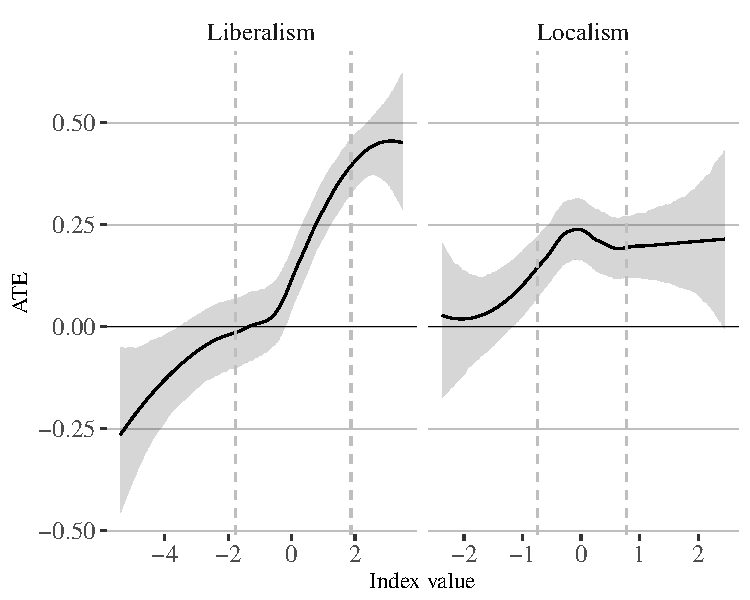
\includegraphics[width=.85\textwidth]{e_ate}
  }  
  \end{measuredfigure}
  \begin{tablenotes}[flushleft]
    \item \hspace{-.2em}\emph{Notes:} The figure shows the average treatment effect (ATE), or the relative preference for the mixed-income project over the high-end project, across a range of liberalism and localism scores.  The ATE corresponds to the difference between the LOESS curves reported in Figure~\ref{fig:hg_e_lib_loc}.  The support (range) for each plot consists of values between the 1st and 99th percentiles for each index.  Shaded areas indicate bootstrapped 95\% confidence intervals. The vertical dashed lines represent the 20th and 80th percentiles for the respective scores.
  \end{tablenotes}
\end{figure}

% -----------------------------------------------------------------------------
% Tab: Lib and loc regressions
% -----------------------------------------------------------------------------
\begin{table}
  \caption{Regressions of Support for Project on Liberalism and Localism}
  \label{tab:hg_e_support_regression}
  \begin{threeparttable}
  \scriptsize
  \begin{tabularx}{\linewidth}{X}
  \centering

  \begin{tabular}{@{\extracolsep{5pt}}lcccc} 
  \\[-1.8ex]\hline 
  \hline \\[-1.8ex] 
   & \multicolumn{4}{c}{\textit{Dependent variable:}} \\ 
  \cline{2-5} 
  \\[-1.8ex] & High-end & Mixed-income & High-end & Mixed-income\\ 
  \\[-1.8ex] & (1) & (2) & (3) & (4)\\ 
  \hline \\[-1.8ex] 
   Liberalism & $-$0.045$^{}$ & 0.050$^{}$ & $-$0.040$^{}$ & 0.049$^{}$ \\ 
    & (0.008) & (0.007) & (0.008) & (0.008) \\ 
    & & & & \\ 
   Liberalism-squared & $-$0.006$^{}$ & $-$0.002 & $-$0.006$^{}$ & $-$0.003 \\ 
    & (0.003) & (0.003) & (0.003) & (0.003) \\ 
    & & & & \\ 
   Localism & $-$0.088$^{}$ & $-$0.041$^{}$ & $-$0.077$^{}$ & $-$0.043$^{}$ \\ 
    & (0.015) & (0.014) & (0.016) & (0.015) \\ 
    & & & & \\ 
   Localism-squared & 0.005 & 0.001 & 0.004 & 0.005 \\ 
    & (0.010) & (0.010) & (0.010) & (0.010) \\ 
    & & & & \\ 
   Female &  &  & $-$0.104$^{}$ & 0.002 \\ 
    &  &  & (0.032) & (0.029) \\ 
    & & & & \\ 
   White &  &  & 0.010 & 0.058$^{}$ \\ 
    &  &  & (0.037) & (0.034) \\ 
    & & & & \\ 
   Age < 35 &  &  & $-$0.022 & 0.010 \\ 
    &  &  & (0.034) & (0.031) \\ 
    & & & & \\ 
   No 4-year college degree &  &  & $-$0.025 & $-$0.008 \\ 
    &  &  & (0.035) & (0.031) \\ 
    & & & & \\ 
   Post-graduate degree &  &  & $-$0.005 & $-$0.035 \\ 
    &  &  & (0.047) & (0.046) \\ 
    & & & & \\ 
   Income < \$60,000 &  &  & $-$0.082$^{}$ & 0.043 \\ 
    &  &  & (0.038) & (0.034) \\ 
    & & & & \\ 
   Income \$100-150,000 &  &  & 0.009 & 0.018 \\ 
    &  &  & (0.055) & (0.049) \\ 
    & & & & \\ 
   Income > \$150,000 &  &  & 0.086 & 0.093 \\ 
    &  &  & (0.078) & (0.082) \\ 
    & & & & \\ 
   Homeowner &  &  & $-$0.013 & $-$0.031 \\ 
    &  &  & (0.036) & (0.032) \\ 
    & & & & \\ 
   Resident > 4 years &  &  & $-$0.032 & $-$0.006 \\ 
    &  &  & (0.035) & (0.031) \\ 
    & & & & \\ 
   5-year HPA > median &  &  & $-$0.033 & 0.007 \\ 
    &  &  & (0.032) & (0.029) \\ 
    & & & & \\ 
   Constant & 0.561$^{}$ & 0.730$^{}$ & 0.720$^{}$ & 0.668$^{}$ \\ 
    & (0.022) & (0.020) & (0.066) & (0.060) \\ 
    & & & & \\ 
  \hline \\[-1.8ex] 
  Observations & 1,007 & 982 & 970 & 971 \\ 
  R$^{2}$ & 0.062 & 0.072 & 0.085 & 0.080 \\ 
  Adjusted R$^{2}$ & 0.058 & 0.068 & 0.071 & 0.066 \\ 
  \hline 
  \hline \\[-1.8ex] 
  \end{tabular}   

  \end{tabularx}
  \begin{tablenotes}[flushleft]
    \item \hspace{-.2em}\emph{Notes:} OLS estimates of linear probability models for project support.
  \end{tablenotes}
  \end{threeparttable}
\end{table}

% -----------------------------------------------------------------------------
% Fig: SFHG scree
% -----------------------------------------------------------------------------
\begin{figure}[htb]\centering
  \caption{Proportion of Variance Explained}
  \label{fig:hg_g_scree}
  \begin{measuredfigure}
  \makebox[\linewidth]{%
  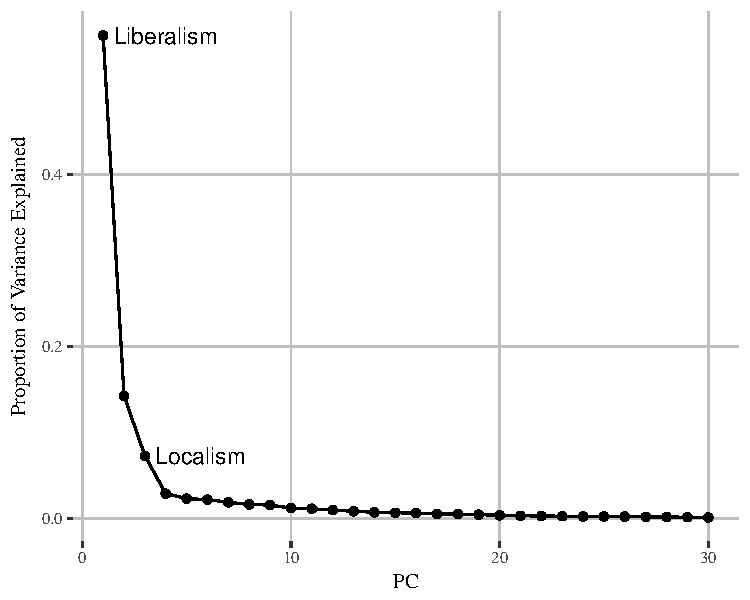
\includegraphics[width=.6\textwidth]{g_scree}
  }  
  \end{measuredfigure}
  \begin{tablenotes}[flushleft]
    \item \hspace{-.2em}\emph{Notes:} The figure shows the proportion of variance explained by each principal component.
  \end{tablenotes}
\end{figure}

% -----------------------------------------------------------------------------
% Map: four types
% -----------------------------------------------------------------------------
\begin{figure}[tb]\centering
  \caption{Geographical Distribution of Political Preferences}
  \label{fig:hg_g_map_types}
  \begin{measuredfigure}
  \makebox[\linewidth]{%
  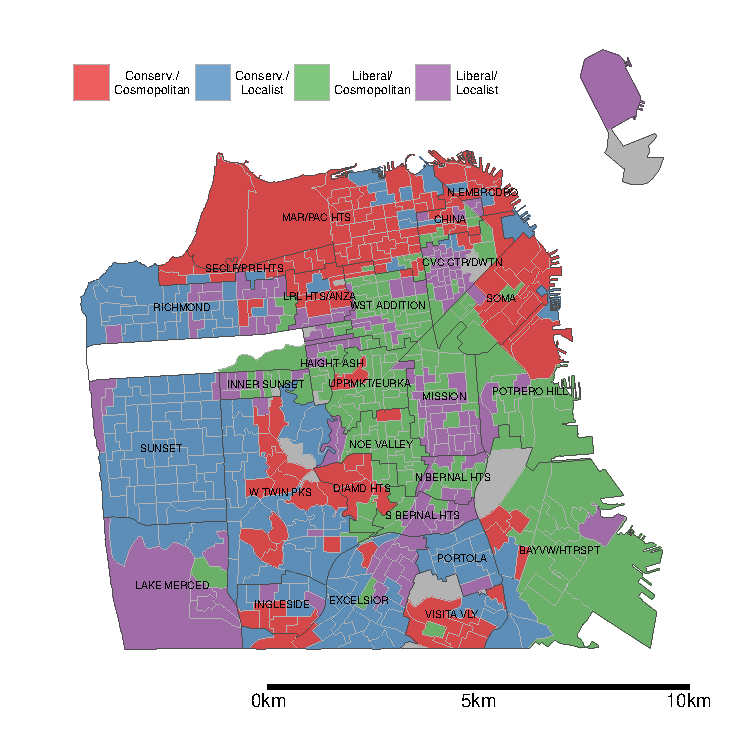
\includegraphics[width=.75\textwidth]{g_map_types}
  }
  \end{measuredfigure}
  \begin{tablenotes}[flushleft]
    \item \hspace{-.2em}\emph{Notes:} The map show the geographic distribution of four categories of political preferences. Precincts are categorized by the interaction of whether they score above or below the median on liberalism (liberal or conservative) and whether they score above or below the median on localism (localist or cosmopolitan).
  \end{tablenotes}
\end{figure}


% -----------------------------------------------------------------------------
% Tab: Regression
% -----------------------------------------------------------------------------
\newgeometry{margin=1.5in} % modify this if you need even more space
\begin{landscape}

\begin{table}
  \caption{Regressions of Support for Project on Localism and Liberalism}
  \label{tab:hg_g_support_regression}
  \begin{threeparttable}
  \scriptsize
  \begin{tabularx}{\linewidth}{X}
  \centering

\begin{tabular}{@{\extracolsep{5pt}}lcccccccc} 
\\[-1.8ex]\hline 
\hline \\[-1.8ex] 
 & \multicolumn{8}{c}{\textit{Dependent variable:}} \\ 
\cline{2-9} 
\\[-1.8ex] & Shipyard & Shipyard & 8 Wash. & 8 Wash. & Pier 70 & Pier 70 & Mis. Rock & Mis. Rock\\ 
\\[-1.8ex] & (1) & (2) & (3) & (4) & (5) & (6) & (7) & (8)\\ 
\hline \\[-1.8ex] 
 Localism & $-$0.027$^{}$ & $-$0.029$^{}$ & $-$0.015$^{}$ & $-$0.018$^{}$ & $-$0.029$^{}$ & $-$0.023$^{}$ & $-$0.026$^{}$ & $-$0.023$^{}$ \\ 
  & (0.005) & (0.005) & (0.008) & (0.008) & (0.005) & (0.005) & (0.004) & (0.003) \\ 
  & & & & & & & & \\ 
 Liberalism & $-$0.061$^{}$ & $-$0.065$^{}$ & $-$0.025$^{}$ & $-$0.030$^{}$ & 0.031$^{}$ & 0.031$^{}$ & 0.032$^{}$ & 0.021$^{}$ \\ 
  & (0.008) & (0.007) & (0.008) & (0.009) & (0.005) & (0.003) & (0.004) & (0.004) \\ 
  & & & & & & & & \\ 
 Constant & 0.628$^{}$ & 0.644$^{}$ & 0.330$^{}$ & 0.356$^{}$ & 0.725$^{}$ & 0.717$^{}$ & 0.739$^{}$ & 0.766$^{}$ \\ 
  & (0.007) & (0.014) & (0.008) & (0.021) & (0.006) & (0.006) & (0.005) & (0.007) \\ 
  & & & & & & & & \\ 
\hline \\[-1.8ex] 
Strata fixed effects & No & Yes & No & Yes & No & Yes & No & Yes \\ 
\hline \\[-1.8ex] 
Observations & 578 & 578 & 578 & 578 & 578 & 578 & 578 & 578 \\ 
R$^{2}$ & 0.580 & 0.602 & 0.179 & 0.257 & 0.496 & 0.606 & 0.531 & 0.643 \\ 
Adjusted R$^{2}$ & 0.579 & 0.595 & 0.176 & 0.243 & 0.495 & 0.599 & 0.529 & 0.637 \\ 
\hline 
\hline \\[-1.8ex] 
\end{tabular}

  \end{tabularx}
  \begin{tablenotes}[flushleft]
    \item \hspace{-.2em}\emph{Notes:} OLS estimates of linear models for project support. Numbers in parentheses report standard errors, clustered by neighborhood. Coefficients for localism and liberalism represent change in vote share for a standard deviation change in the predictor value. Strata are generated by first computing terciles for precinct-level median household income and precinct-level homeownership rates, then interacting both categorical variables to form nine cells. Household income and homeownership rates come from the 2010 Census, and are imputed to precincts from Census geographies using conversion tables from the Statewide Database, available at \url{http://statewidedatabase.org/conversion.html}.
  \end{tablenotes}
  \end{threeparttable}
\end{table}

\end{landscape}
\restoregeometry

\end{SingleSpacing}

\end{document}